%%% lecture notes class
\documentclass{llncs}

%%% basic packages %%%
\usepackage[T1]{fontenc} 
\usepackage{tgtermes}
\usepackage{amssymb}
\usepackage{amsmath}
\usepackage{graphicx}
\usepackage{esint}
\usepackage{enumitem}
\usepackage{algorithm}
\usepackage{hyperref}
\usepackage{marvosym}
\usepackage{mathtools}
\usepackage{xspace} 
\usepackage{color}
\usepackage{comment}

%%% some custom stuff %%%
\usepackage[noend]{algpseudocode}
\usepackage[section]{placeins}
\usepackage{hyperref}
\renewcommand\algorithmicthen{}
\renewcommand\algorithmicdo{}
\algrenewcommand\algorithmicindent{1.0em}
\newenvironment{megaalgorithm}[1][htb]
  {\renewcommand{\algorithmcfname}{MegaAlgorithm}
   \begin{algorithm}[#1]
  }{\end{algorithm}}

%%% Words %%%
\newcommand{\GLC}{\ensuremath{\mathrm{GLC}}\xspace}
\newcommand{\PRM}{\ensuremath{\mathrm{PRM}}\xspace}
\newcommand{\PRMs}{\ensuremath{\mathrm{PRM}^*}\xspace}
\newcommand{\RRT}{\ensuremath{\mathrm{RRT}}\xspace}
\newcommand{\RRTs}{\ensuremath{\mathrm{RRT}^*}\xspace}
\newcommand{\SST}{\ensuremath{\mathrm{SST}}\xspace}
\newcommand{\EST}{\ensuremath{\mathrm{EST}}\xspace}
\newcommand{\NULL}{\ensuremath{\mathtt{NULL}}\xspace}

\setlength{\marginparwidth}{1in}
\newcommand{\efmargin}[2]{{\color{blue}#1}\marginpar{\raggedright\footnotesize\color{blue}[EF] #2}}
% Uncomment the line below to remove efmargin notes
%\renewcommand{\efmargin}[2]{{#1}}

\begin{document}
\title{A Generalized Label Correcting Method for \\ Optimal Kinodynamic Motion Planning }

\author{Brian Paden and Emilio Frazzoli}
\institute{Massachusetts Institute of Technology \\ 
\email{bapaden@mit.edu}, $\quad$ \email{frazzoli@mit.edu}}
\maketitle
\begin{abstract}
%
An optimal kinodynamic motion planning algorithm is presented and  described as a generalized label correcting (\GLC) method.
%
%In contrast to related algorithms, the \GLC  method does not require a local planning subroutine and relies on weaker technical assumptions.
%
Advantages of the technique include a simple implementation, convergence to the optimal cost with increasing resolution, and no requirement for a point-to-point local planning subroutine.
%
The principal contribution of this paper is the construction and analysis of the \GLC conditions which are the basis of the proposed algorithm.
%
%Numerical experiments demonstrate the \GLC method is suitable for real-time optimal motion planning in up to six dimensional state spaces.
%
%

\end{abstract}
%

\section{Introduction}
%%%%%New%%%%%
Motion planning is a challenging and fundamental problem in robotics research with numerous algorithms fine-tuned to variations of the problem.
%

%
Among the most popular is the \PRM~\cite{PRM}, an algorithm for planning in relatively high dimensions, but requires a point-to-point local planning subroutine or steering function to connect pairs of randomly sampled states.
%
A variation, \PRMs~\cite{karaman2011sampling}, converges to an optimal solution with respect to some objective provided the steering function is optimal.
%
%Local planning subroutines are often unavailable for differentially constrained systems.

%
The \EST~\cite{EST_Journal} and \RRT~\cite{RRT_Journal} algorithms were developed to address problems with differential constraints where a steering function is unavailable.
%
The steering function in these algorithms is replaced by a subroutine which forward integrates the system dynamics with a selected control input.
%

%
Optimal planning under differential constraints can be addressed by the kinodynamic variant of the \RRTs algorithm~\cite{karaman2010optimal}, but again requires an optimal steering function like \PRMs. 
%
The effectiveness of \RRTs has motivated several general approaches for optimal steering discussed in~\cite{perez2012lqr,xie2015toward}.
%
However, the computation of these solutions can slow down the iteration time of \RRTs considerably.
%

%
%Like \RRT and \EST, the recently developed \SST algorithmuses forward integration instead of local steering, but provides almost sure convergence to an approximately optimal solution.
%
%The use of forward integration instead of a steering function makes \SST applicable to many more problems than the kinodynamic \RRTs algorithm. 
%

%
This paper addresses optimal planning under differential constraints without the use of a steering function. 
%
The method is based on a discrete approximation of the problem as a graph together with a generalization of label correcting techniques such as Dijkstra's algorithm~\cite{dijkstra1959note}.
%

%
Label correcting algorithms compare the relative cost of paths in a graph terminating at the same vertex and discard paths with non-minimal cost.
%
This is effective when there are multiple paths reaching each vertex from the root vertex.
%
Without a steering function it is difficult to construct such a graph approximating motion planning solutions since multiple trajectories terminating at specified states must be generated.
%
The intuitive generalization is to compare the cost of paths related to trajectories terminating "close enough" to one another.
%
An ad hoc implementation of this concept first appeared in~\cite{fox1998hybrid} as the Hybrid $\rm A^*$ algorithm.
%
More recently, the \SST algorithm~\cite{Li2016Asymptotically-} provided a more principled approximation of the problem and an algorithm converging asymptotically to a solution with bounded sub-optimality. 
%
 
%
%A conventional label correcting algorithm compares the cost of paths terminating at the same vertex of a graph and discards the path with greater cost. 
%
%To benefit from this operation, a graph approximating a motion planning problem must have a number of paths terminating at each vertex.
%
%Building such a graph requires an exact steering function. 
%
%A natural generalization which does not require exact steering is to compare trajectories terminating in the same region of the state space. 
%
%This concept is applied in~\cite{fox1998hybrid} as the Hybrid $\rm A^*$ algorithm and more recently in ~\cite{Li2016Asymptotically-} as the \SST algorithm.  
%

%
%The Hybrid $\rm A^*$ algorithm uses an ad hoc approximation of the problem without theoretical guarantees on the quality of the solution.
%
%In contrast, \SST algorithm was proven to converge to a solution with bounded sub-optimality given infinite running time.
%
This paper refines this approach further with an algorithm producing solutions with bounded sub-optimality and terminating in finite-time. 
%
The key difference allowing the algorithm to terminate in finite time is a slightly more conservative comparison between paths terminating in the same region of the state space. 
%
This comparison is described in Section \ref{sec:GLC-Methods}.
%
Section \ref{sec:Numerical-Examples} provides examples illustrating convergence to optimal cost solutions with increasing resolution. 
%
The analysis of the algorithm is addressed Section \ref{sec:Justification} and is the principal contribution of the paper.
%

%They provide a pruning condition for the search tree that does not compromise optimality.
%
%Although grid-based methods are taboo in the sampling-based literature, the experiments  
%
%Section \ref{sec:Justification}, provides the analysis proving the proposed \GLC method is a resolution complete optimal kinodynamic motion planning algorithm. 

\begin{comment}
%%%%%Old%%%%%
Motion planning is one of the most fundamental and challenging problems in robotics providing a system with the capability to autonomously decide on motions to perform a task.
%
The importance of this problem has stimulated decades of research.
%

%
A major breakthrough was the introduction of the \PRM~\cite{PRM}, a probabilistically complete algorithm for planning in general environments.
%
The approach relies on two subroutines to be applied on a particular system.
%
The first is a feasibility checking module for candidate motions. 
%
The second is a local planner to generate trajectories connecting two configurations or states.
%

%
For systems with differential constraints, an exact local planner is often unavailable.
%
In these instances the term kinodynamic is added to emphasize that both kinematic and differential constraints must be taken into account. 
%
The \RRT~\cite{RRT_Journal} method was introduced to address this challenge.
%
Instead of exact local planning, \RRT requires an approximate local planner to provide a trajectory whose terminal state is closer to the randomly sampled state than the initial state.
%
%While \RRT works well in practice, the assumptions required to guarantee probabilistic completeness are difficult to verify from problem data.
%
The \EST~\cite{EST_Journal} method, introduced shortly thereafter, is similar in priciple to \RRT but extends the search by forward integrating random inputs. 
%
 
%
While these methods are effective for planning feasible motions, solutions tend to be poor in quality. The \RRTs~\cite{karaman2011sampling} method was developed as an optimal variant to \RRT.
%
However, in addition to the collision checking module, \RRTs requires an \textit{optimal} local planner. 
%
To address this limitation, a number of approaches for efficient local planning have been proposed~\cite{perez2012lqr,xie2015toward,stoneman2014embedding}.
%
However, \RRTs is most effective when the local planner is available as a closed form solution. 
%

%
More recently, the \SST~\cite{Li2016Asymptotically-} algorithm was developed providing almost sure asymptotic convergence to an approximately optimal solution without the use of a local planner. It is arguably the most general purpose planning algorithm available.
%

%
In this paper we present a novel framework which generalizes classical label correcting techniques such as Dijkstra's algorithm~\cite{dijkstra1959note}. 
%
We propose an algorithm which under mild assumptions returns a feasible approximation of an optimal solution in finite time. 
%
This new approach and the key observations which we call the \GLC conditions are introduced in Section \ref{sec:GLC-Methods}. 
%
An implementation of the algorithm was tested in several numerical experiments in Section \ref{sec:Numerical-Examples} to make a comparison with the \SST and \RRTs algorithms.
%
Section \ref{sec:Justification}, provides the analysis proving the proposed \GLC method is a resolution complete optimal kinodynamic motion planning algorithm.
\end{comment} 
\section{\label{sec:GLC-Methods}GLC Methods}

\paragraph{Label correcting methods:}
Shortest path algorithms are methods of searching over paths of a graph for a minimum-cost path between an origin or root vertex to a set of goal vertices.
% 
In a conventional label correcting method, the algorithm maintains a best known path terminating at each vertex of the graph. This path \textit{labels} that vertex. 
%
At a particular iteration, if a path under consideration does not have lower cost than the path labeling the terminal vertex, the path under consideration is discarded. 
%
As a consequence, the subtree of paths originating from the discarded path will not be evaluated.

%Justification for this operation is that any concatenation of edges with the discarded path can also be concatenated with the path labeling the vertex to obtain a path of equal or lesser cost.
%
%This can be interpreted as forward dynamic programming~\cite[pg. 77]{bertsekas1995dynamic}.

\paragraph{Generalizing the notion of a label:}
Observe that the label of a vertex in conventional label correcting algorithms is in fact a label for the paths terminating at that vertex.
%
Then each vertex identifies an equivalence class of paths.
% 
Paths within each equivalence class are ordered by their cost, and the efficiency of label correcting methods comes from narrowing the search to minimum cost paths in their associated equivalence class. 
% 
The generalization is to identify paths associated to trajectories terminating in the same region of the state space instead of the same state.
%
However, this generalization prevents a direct comparison of cost between two related paths. 
%
Instead, the difference in cost must exceed a threshold  described by the \GLC conditions introduced in Section \ref{sec:glc_def}. 


\subsection{Problem Formulation}

Consider a system whose configuration and relevant quantities are described by a state in $\mathbb{R}^{n}$. 
%
The decision variable of the problem is an input signal or continuous history of actions $u$ from a \textit{signal space} $\mathcal{U}$ affecting a state trajectory $x$ in a \textit{trajectory space} $\mathcal{X}_{x_0}$. The signal space is constructed from a set of admissible inputs $\Omega\subset\mathbb{R}^{m}$ bounded by $u_{max}$. The input signal space is defined
%
\begin{equation}
\mathcal{U}\coloneqq\bigcup_{\tau>0}\left\{ u\in L_{1}([0,\tau]):\: u(t)\in\Omega\:\,\forall t\in[0,\tau]\right\}. \label{eq:signal_space}
\end{equation}

%
The signal and trajectory are related through a model of the system dynamics described by a differential
constraint,
% 
\begin{equation}
\frac{d}{dt}x(t)=f(x(t),u(t)), \quad x(0)=x_0\label{eq:dynamics}.
\end{equation}
%
A \textit{system map} $\varphi_{x_0}:\mathcal{U}\rightarrow\mathcal{X}_{x_0}$ is defined to relate signals to associated trajectories (the solution to (\ref{eq:dynamics})~\cite[cf. pg. 42]{coddington1955theory}) with domain equal to the domain of the input signal. 
%
The initial state $x_0$ parametrizes the map and trajectory space. 
%
To simplify notation, $\tau(x)$ for a function $x$ with domain $[t_1,t_2]$ denotes the maximum of the domain, $t_2$.   

In addition to the differential constraint, feasible trajectories for a particular problem must satisfy point-wise constraints defined by a subset $X_\mathrm{free}$ of $\mathbb{R}^n$ and a specified initial state $x_\mathrm{ic}$. 
%
%Therefore, a feasible trajectory belongs to a subset of $\mathcal{X}_{x_\mathrm{ic}}$ such that $x(t)\in X_\mathrm{free}$ for all $t\in[0,\tau(x)]$.
The subset of feasible trajectories $\mathcal{X}_\mathrm{feas}$ are defined 
%
\begin{equation}
\mathcal{X}_\mathrm{feas}\coloneqq \left\{ x\in \mathcal{X}_{x_\mathrm{ic}}:\,\, x(t)\in X_\mathrm{free}\,\, \forall t\in [0,\tau (x)] \right\}.
\end{equation}
%
Similarly, the subset $X_\mathrm{goal}$ of $\mathbb{R}^n$  is used to encode a terminal constraint. The subset of $\mathcal{X}_\mathrm{feas}$ consisting of trajectories $x$ with $x(\tau(x))\in X_\mathrm{goal}$ defines $\mathcal{X}_\mathrm{goal}$.
%
%The subset of feasible trajectories reaching the goal $\mathcal{X}_\mathrm{goal}$ is defined as
% 
%\begin{equation}
%\mathcal{X}_\mathrm{goal}\coloneqq \left\{ x\in %\mathcal{X}_\mathrm{feas}:\,\, x(\tau(x))\in X_\mathrm{goal}\right\}.
%\end{equation}
%

%
The decision variable for the problem is the input signal $u$ which must be chosen such that the trajectory $\varphi_{x_\mathrm{ic}}(u)$ is in $\mathcal{X}_\mathrm{goal}$.
%
Naturally, input signals mapping to trajectories in $\mathcal{X}_\mathrm{feas/goal}$ are defined by the inverse relation  $\mathcal{U}_\mathrm{feas/goal} \coloneqq \varphi_{x_\mathrm{ic}}^{-1}(\mathcal{X}_\mathrm{feas/goal})$. 

A general cost functional which integrates a running-cost $g$ of the state and input at each instant along a trajectory is used to compare the merit of one input signal over another.
%
Restricted to solutions of (\ref{eq:dynamics}), the cost functional depends only on the control and intitial state, 
%
\begin{equation}
J_{x_{0}}(u)=\int_{[0,\tau(u)]}g([\varphi_{x_{0}}(u)](t),u(t))\, d\mu(t).\label{eq:real_cost}
\end{equation}
%
The notation $[\varphi_{x_{0}}(u)](t)$ denotes the evaluation of the trajectory satisfying (\ref{eq:dynamics}) with the input signal $u$ and initial state $x_{0}$ at time $t$. 

The domain of $J$ is extended with the object \NULL such that $J_{x_0}(\NULL)=\infty$ for all $x_0\in\mathbb{R}^{n}$.
%
Further, since (\ref{eq:real_cost}) may not admit a minimum, we address the following relaxed optimal kinodynamic motion planning problem:
% 
\begin{problem}\label{Problem}
Find a sequence $\{u_{R}\}\subset\mathcal{U}_\mathrm{goal}\cup \NULL$ such that 
%
\begin{equation}
\lim_{R\rightarrow\infty}J_{x_\mathrm{ic}}(u_R)=\inf_{u\in\mathcal{U}_\mathrm{goal}}J_{x_\mathrm{ic}}(u)\coloneqq c^{*}.\label{eq:meaningful_problem}
\end{equation}
%
With the convention that $\inf_{u\in\emptyset}J_{x_\mathrm{ic}}(u)=\infty$, a solution sequence exists so the problem is well-posed. An algorithm parameterized by a resolution $R \in \mathbb{N}$ whose output for each $R$ forms a sequence solving this problem will be called \textit{resolution complete}.
\end{problem}

\paragraph{Assumptions.} The problem data are assumed to satisfy  the following:
%
\begin{enumerate}[label=\textbf{A-\arabic*},itemindent=0.25cm] 
%
\item The sets $X_\mathrm{free}$ and $X_\mathrm{goal}$ are open with respect to the standard topology on $\mathbb{R}^n$.
%
\item There are known constants $L_{f}\geq0$ and $M\geq0$ such that $\left\Vert f(x_{1},u)-f(x_{2},u)\right\Vert _{2}\leq L_{f}\left\Vert \left(x_{1}-x_{2}\right)\right\Vert _{2}$, and $\left\Vert f(x_{1},u)\right\Vert _{2}\leq M$ for all $x_{1},x_{2}\in X_\mathrm{free}$ and $u\in\Omega$.
%
\item  There is a known constant $L_{g}\geq0$ such that $\left\Vert g(x_{1},u_{1})-g(x_{2},u_{2})\right\Vert _{2}\leq$\\$ L_{g}\left\Vert \left(x_{1}-x_{2},u_{1}-u_{2}\right)\right\Vert _{2}$ for all $x_{1},x_{2}\in X_\mathrm{free}$ and $u_{1},u_{2}\in\Omega$.
%
\item  $ J_{x_{ic}}(u)>0 $ for all $u\in\mathcal{U}$.
%
\end{enumerate} 
%

\remark{
%We have assumed that $g$ is Lipschitz continuous whereas \SST makes this assumption for $J$. 
%
%This difference is what enables the \GLC method to compute an approximate solution in finite time.
%

%\RRTs and \SST both require that when a problem is feasible there exist a trajectory passing through the interior of $X_\mathrm{free}$ terminating in $X_\mathrm{goal}$. 
%
%The analogue in our work is that the interior of $\mathcal{U}_\mathrm{goal}$ be nonempty with respect to a topology defined in Section \ref{sec:Justification}. 
%
We do not require the reachable set to have a nonempty interior as in the kinodynamic variant of \RRTs~\cite{karaman2010optimal} and \SST~\cite{Li2016Asymptotically-}.
%
}


\subsection{Approximation of $\mathcal{U}$}


The signal space $\mathcal{U}$ is approximated by a finite subset  $\mathcal{U}_{R}$ where $R\in\mathcal{\mathbb{N}}$ is a resolution parameter. 
%
To construct $\mathcal{U}_{R}$ it is assumed that we have access to a family of finite subsets $\Omega_{R}\subset\Omega$ of the input space, such that the dispersion
%\footnote{The radius of the largest open sphere contained in $\Omega$ whose intersection with $\Omega_R$  is empty.} of $\Omega_{R}$ 
in $\Omega$ converges to zero as $R\rightarrow \infty$. 
%
A family of such subsets exists and is often easily obtained with regular grids or random sampling for a given $\Omega$.   

The approximated signal space $\mathcal{U}_R$ consists of piecewise constant signals on time intervals $\left[\frac{c\cdot(i-1)}{R},\frac{c\cdot i}{R}\right)$ for $c>0$, $i\in\{1,...,d\}$, and all values $d$ less than a user specified function $h(R)$ (take the last interval to be closed). The constant values of the signal are inputs from $\Omega_R$.   

%
The function $h:\mathbb{N}\rightarrow\mathbb{N}$ defines a horizon limit and can be \textit{any} function satisfying
% 
\begin{equation}
\lim_{R\rightarrow\infty}R/h(R)=0.\label{eq:h_constraint}
\end{equation}
%
For example, $h(R)=R\log(R)$ is acceptable. 
%
This ensures that the horizon limit is unbounded in $R$ so that any finite time domain can be approximated for sufficiently large $R$.
%

%
A \textit{parent} of an input signal $w\in\mathcal{U}_{R}$ with domain $\left[0,\frac{c\cdot i}{R}\right]$ is defined as the input signal $u\in\mathcal{U}_{R}$ with domain $\left[0,\frac{c\cdot(i-1)}{R}\right]$ such that $w(t)=u(t)$ for all $t\in\left[0,\frac{c\cdot(i-1)}{R}\right)$.
%
In this case, $w$ is a \textit{child} of $u$. 
%
A tree (graph) is defined with $\mathcal{U}_{R}$ as the vertex set, and edges defined by ordered pairs of signals $(u,w)$ such that $u$ is the parent of $w$.
%
To serve as the root of the tree, $\mathcal{U}_R$ is augmented with the special input signal $Id_{\mathcal{U}}$ defined such that $J_{x_0}(Id_{\mathcal{U}})=0$ and $[\varphi_{x_0}(Id_\mathcal{U})](0)=x_0$. $Id_{\mathcal{U}}$ has no parent, but is the parent of signals with domain $[0,c/R]$. 
%

The signal $w$ is an \textit{ancestor} of $u$ if $\tau(w)<\tau(u)$ and $w(t)=u(t)$ for all $t\in[0,\tau(w))$.
%
In this case $u$ is a \textit{descendant} of $w$. The \textit{depth} of a control in $\mathcal{U}_{R}$ is the number of ancestors of that control.

\subsection{Partitioning $X_\mathrm{free}$ and the GLC Conditions}
\label{sec:glc_def}
%The \GLC conditions define a partial order on $\mathcal{U}_R$ that represents some notion of relative quality between comparable signals. 
%
%The idea is to discard a signal if it is greater than another. 
%
A partition of $X_\mathrm{free}$ is used to define comparable signals. We say the partition has radius $r$ if the partition elements are each contained in a neighborhood of radius $r$.
%
Like the discretization of $\mathcal{U}$, the radius of the partition is parametrized by the resolution $R$. 

%
For brevity we only consider hypercube partitions.
%
A user specified function $\eta:\mathbb{N}\rightarrow\mathbb{R}_{>0}$ controls the side length of the hypercube. 
%
For states $p_1,p_2\in\mathbb{R}^n$ we write $p_1\overset{R}{\sim}p_2$ if $\left\lfloor \eta(R)p_1\right\rfloor =\left\lfloor \eta(R)p_2\right\rfloor$, where $\left\lfloor \cdot\right\rfloor $ is the coordinate-wise floor map (e.g. $\left\lfloor (2.9,3.2) \right\rfloor = (2,3)$). 
%
Then the equivalence classes of the $\overset{R}\sim$ relation define a simple hypercube partition of radius $\sqrt{n}/\eta(R)$.    
%
We extend this relation to control inputs by comparing the terminal state of the resulting trajectory. 
%
For $u_1,u_2 \in \mathcal{U}_R$ we write $u_{1}\overset{\mathcal{U}_R}{\sim}u_{2}$ if the resulting trajectories terminate in the same hypercube. That is,
%
\begin{equation}\label{eq:equiv_signal}
u_{1}\overset{\mathcal{U}_R}{\sim}u_{2} \Leftrightarrow [\varphi_{x_\mathrm{ic}}(u_{1})](\tau(u_{1})) \overset{R}{\sim}  [\varphi_{x_\mathrm{ic}}(u_{2})](\tau(u_{2})) .
\end{equation}
%
Figure \ref{fig:intuition} illustrates the intuition behind this equivalence relation.
%
%We propose the \GLC method as for identifying and labeling the equivalence classes of $\overset{\mathcal{U}_R}\sim$.
%
%\GLC conditions define a partial ordering $\prec_{R}$ on $\mathcal{U}_{R}$ which is used to quantify which signals can be discarded. 
%

%
To compare signals we write $u_{1}\prec_{R}u_{2}$ if the \GLC conditions are satisfied:
%
\begin{enumerate}[label=\textbf{GLC-\arabic*},itemindent=0.75cm] 
\item \label{glc1} $u_{1}\overset{\mathcal{U}_R}\sim u_{2}$,
\item \label{glc2} $\tau(u_{1})\leq\tau(u_{2}),$
\item \label{glc3} $J_{x_\mathrm{ic}}(u_{1})+\frac{\sqrt{n}}{\eta(R)}\frac{L_{g}}{L_{f}}\left(e^{\frac{L_{f}h(R)}{R}}-1\right) \leq J_{x_\mathrm{ic}}(u_{2}).$
\end{enumerate}
%
A signal $u_1$ is called \textit{minimal} if there is no $u_2\in \mathcal{U}_R$ such that $u_{2}\prec_{R}u_{1}$. Such a signal can be thought of as being a good candidate for later expansion during the search. Otherwise, it can be discarded.
%
In order for the \GLC method to be a resolution complete algorithm, the scaling parameter $\eta$ must satisfy  
%
\begin{equation}
\lim_{R\rightarrow\infty}\frac{R}{L_f\eta(R)}\left(e^{\frac{L_{f}h(R)}{R}}-1\right)=0.\label{eq:partition_scaling}
\end{equation}
%  
%it is sufficient for a resolution complete algorithm to systematically examine minim\underline{al} signals in $\mathcal{U}_R$ in the same way that classical label correcting methods need only examine minim\underline{um} cost paths of each equivalence class. 
%
%The cardinality of $\mathcal{U}_R$ is nominally much greater than the cardinality of its minimal elements so that searching only minimal elements affords savings in computation.
%  

%
Observe that (\ref{eq:partition_scaling}) implies the cost threshold in \ref{glc3} is in $O(1/R)$ and converges to zero.
%
A condition yielding the same theoretical results, but asymptotically requiring more signals to be evaluated would be to replace the threshold with an arbitrarily small positive constant. 
%

%
Additionally, (\ref{eq:partition_scaling}) and \ref{glc3} simplify in some cases.
%
For kinematic problems $L_{f}=0$.
%
Taking the limit $L_{f}\rightarrow 0$, the constraint (\ref{eq:partition_scaling}) becomes $h(R)/\eta(R)\rightarrow 0$.
%
The second special case is minimum-time problems where $g(x,u)=1$ in (\ref{eq:real_cost}) so that $L_{g}=0$. 
%
Then \ref{glc3} simplifies to $J_{x_\mathrm{ic}}(u_{1}) \leq J_{x_\mathrm{ic}}(u_{2})$.

\begin{figure}[htb]
\centering{}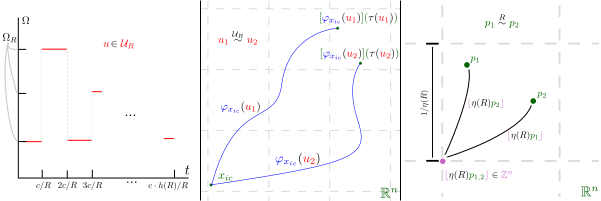
\includegraphics[width=1\textwidth]{Graphics/Theory_Intuition/intuition}
\caption{\label{fig:intuition} Color coded depictions of: (left) a signal from $\mathcal{U}_R$ with signals represented in red, (middle) the mapping into the trajectory space $\mathcal{X}_{x_\mathrm{ic}}$ in blue for two equivalent signals $u_1 \overset{\mathcal{U}_R}{\sim}u_2$, and (right) the mapping from terminal states in $\mathbb{R}^n$ shown in green into $\mathbb{Z}^n$ by the floor map.}
\end{figure}

\subsection{Algorithm Description} 

Pseudocode for the \GLC method is described in Algorithm \ref{Alg} below. A set $Q$ serves as a priority queue of candidate signals. A set $\Sigma$ contains signals representing labels of $\overset{\mathcal{U}_R}{\sim}$ equivalence classes.

The method $expand(u)$ returns the set of all children of $u$. 
%
The method $pop(Q)$ deletes from Q, and returns an input signal $\hat{u}$ such that 
%
\begin{equation}
\hat{u}\in\underset{u\in Q}{{\rm argmin}}\left\{ J_{x_\mathrm{ic}}(u)\right\}. \label{eq:queue}
\end{equation} 
%
The addition of an admissible heuristic~\cite{hart1968formal} in (\ref{eq:queue}) can be used to guide the search without affecting the solution accuracy.  

The method $find(u,\Sigma)$ returns $w\in\Sigma$ such that $u\overset{R}{\sim}w$ or \NULL if no such $w$ is present in $\Sigma$.
%
Problem specific collision and goal checking subroutines are used to evaluate $u\in\mathcal{U}_\mathrm{feas}$ and $u\in\mathcal{U}_\mathrm{goal}$.
%
The method $depth(u)$ returns the number of ancestors of $u$. 
%
\begin{algorithm} 
\begin{algorithmic}[1]
\State $Q\leftarrow \{Id_\mathcal{U}\},\,\Sigma \gets \emptyset,\,S \gets \emptyset$  
\While {$Q\neq \emptyset$}        
\State $u \gets pop(Q)$   
\State $S \gets expand(u)$   
\For{$w \in S$} 	
\If{$w \in \mathcal{U}_\mathrm{goal} $}         	  
\State \Return $(J_{x_{ic}}(w),w)$ 	
\EndIf       
\State $z = find(w,\Sigma)$ 	  
\If{$(w \notin \mathcal{U}_{feas.} \vee (z \prec_R w) \vee depth(w) \geq h(R))$}  	    
\State $S \gets S\setminus \{w\}$  	  
\ElsIf{$J_{x_\mathrm{ic}}(w)<J_{x_\mathrm{ic}}(z)$} 	  
\State $\Sigma \gets (\Sigma \setminus \{z\}) \cup \{w\}$ 	  
\EndIf 
\EndFor       
\State $Q \gets Q \cup S$ 
\EndWhile  
\State 
\Return $(\infty,\NULL)$ 
\end{algorithmic} \caption{\label{Alg} Generalized Label Correcting (GLC) Method} 
\end{algorithm}
%

%
The algorithm begins by adding the root $Id_\mathcal{U}$ to the queue (line 1), and then enters a loop which recursively removes and expands the top of the queue (line 3) adding children to $S$ (line 4). 
%
If the queue is empty the algorithm terminates (line 2) returning \NULL (line 14). 
%
Each signal in $S$ (line 5) is checked for membership in $\mathcal{U}_\mathrm{goal}$ in which case the algorithm terminates returning a feasible solution with approximately the optimal cost. 
%
Otherwise, the signals are checked for infeasibility or suboptimality by the \GLC conditions (line 9). 
%
Next, a relabeling condition for the associated equivalence classes (i.e. grid cells) of remaining signals is checked (line 11). 
%
Finally, remaining signals in $S$ are added to the queue (line 13).  
%
%\begin{figure}[htb]%
%	\centering{}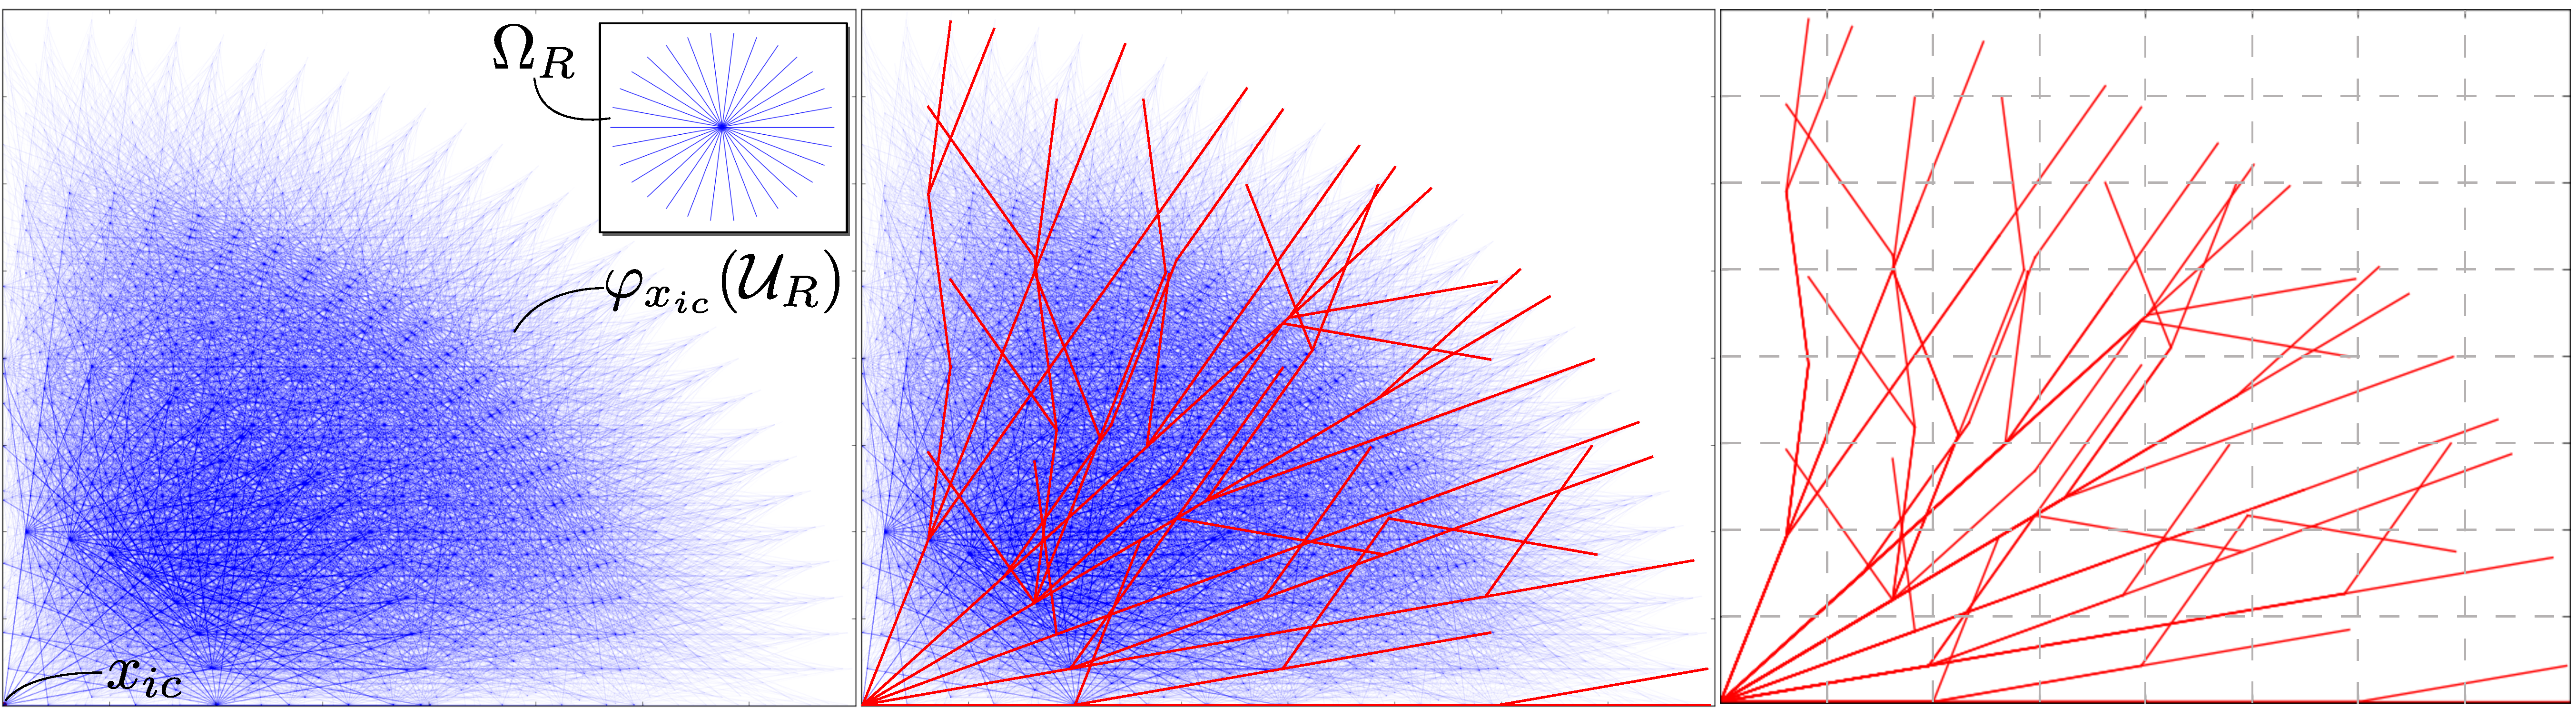
\includegraphics[width=1\textwidth]{Graphics/more_intuition/intuition2}
%	\caption{\label{fig:intuition2} (left) A 2D enviroment illustrating $66,781$ paths defined by exhaustively evaluating $\mathcal{U}_R$. (center) Of these, Algorithm \ref{Alg} evaluates a sub-tree of $57$ paths. (right) Illustration of the grid partitioning the 2D environment.}
%\end{figure}

%
The main result of this paper, justified in Section \ref{sec:Justification}, is the following:
\begin{theorem}\label{thm:informal}
	Let $w_R$ be the signal returned by the \GLC method for resolution $R$. Then $\lim_{R\rightarrow \infty} J_{x_{ic}}(w_R)=c^*$. That is, the \GLC method is a resolution complete algorithm for the optimal kinodynamic motion planning problem.
\end{theorem}
% 
This conclusion is independent of the order in which children of the current node are examined in line 5 as well as the relabeling condition in line 11. 

%Figure \ref{fig:intuition2} is a conceptual illustration of the subset of $\mathcal{U}_R$ evaluated by the algorithm. 
%
%At a fixed resolution the algorithm is a standard grid search, 
%
%The novelty of the GLC method is that a single parameter governs the approximation of the problem and the graph search for a broad class of systems and cost functions.   

\section{\label{sec:Numerical-Examples}Numerical Experiments}

The \GLC method (Algorithm \ref{Alg}) was tested on five problems and compared, when applicable, to the implementation of \RRTs from~\cite{rrt_implementation} and \SST from~\cite{BBekris2015}. 
%
The goal is to examine the performance of the \GLC method on a wide variety of problems. 
%
The examples include under-actuated nonlinear systems, multiple cost objectives, and environments with/without obstacles.
%
Note that adding obstacles effectively speeds up the \GLC method since it reduces the size of the search tree.
%

%
Another focus of the examples is on real-time application.
%
In each example the running time for \GLC method to produce a (visually) acceptable trajectory is comparable to the execution time.
%
Of course this will vary with problem data and computing hardware.    

\paragraph{Implementation Details:}

The \GLC method was implemented in C++ and run with a 3.70GHz Intel Xeon CPU. 
%
The set $Q$ was implemented with an STL priority queue so that the $pop(Q)$ method and insertion operations have logarithmic complexity. 
%
The set $\Sigma$ was implemented with an STL set which uses a binary search tree so that $find(w,\Sigma)$ has logarithmic complexity as well. 
%

Sets $X_\mathrm{free}$ and $X_\mathrm{goal}$ are described by algebraic inequalities.
%
The approximation of the input space $\Omega_{R}$ is constructed by uniformly sampling $R^{m}$ controls from $\Omega$.
%
Recall $m$ is the dimension of the input space. 


Evaluation of $u\in\mathcal{U}_\mathrm{feas}$ and $u\in\mathcal{U}_\mathrm{goal}$ is approximated by first numerically approximating $\varphi_{x_\mathrm{ic}}(u)$ with Euler integration (except for \RRTs which uniformly samples along the local planning solution). 
%
The number of time-steps is given by $N=\left\lceil \tau(u)/\Delta\right\rceil $ with duration $\tau(u)/N$. Maximum time-steps $\Delta$ are 0.005 for the first problem, 0.1 for the second through fourth problem, and 0.02 for the last problem. Feasibility is then approximated by collision checking at each time-step along the trajectory.
%

\paragraph*{Shortest path problem: }

A shortest path problem can be represented by the dynamics $f(x,u)=u$ with the running-cost $g(x,u)=1$ and input space $\Omega=\{u\in\mathbb{R}^{2}:\,\Vert u\Vert_{2}=1\}.$
The free space and goal are illustrated in Figure \ref{fig:bench}.
%
The parameters for the \GLC method are $c=10$, $\eta(R)=300R^2$, and $h(R)=100R\log(R)$ with resolutions $R\in \{20,25,...,200\}$.
%
The exact solution to this problem is known so we can compare the relative convergence rates of the \GLC method, \SST, and \RRTs. 

\paragraph*{Torque limited pendulum swing-up: }

The system dynamics are $f(\theta,\omega,u)=(\omega,u-\sin(\theta))^{T}$
with the running-cost $g(\theta,\omega,u)=1$ and input space  $\Omega=[-0.2,0.2]$.
The free space is modeled as $X_{free}=\mathbb{R}^2$.
%
The initial state is $x_{ic}=(0,0)$ and the goal region is $X_{goal}=\{x\in \mathbb{R}^2:\,\Vert(\theta \pm \pi,\omega \Vert_2 \leq 0.1\}$. 
%
The parameters for the \GLC method are $c=6$, $\eta(R)=16R^{2.5}$, and $h(R)=100R\log(R)$ with resolutions $R\in \{4,5,6,7,8\}$.
%
The optimal solution is unknown so only the running time vs. cost can be plotted. 
%
Without a local planning solution \RRTs is not applicable. 
%
The same is true for the remaining examples.


\paragraph*{Torque limited acrobot swing-up: }

The acrobot is a double link pendulum actuated at the middle joint. 
%
The expression for the four dimensional system dynamics are cumbersome to describe and we refer to~\cite{spong1995swing} for the details. 
%
The model parameters, free space, and goal region are identical to those in \cite{BBekris2015} with the exception that the radius of the goal region is reduced to 0.5 from 2.0.
%
The running-cost is $g(x,u)=1$ and the input space is $\Omega=[-4.0,4.0]$. 
%
The parameters for the \GLC method are $c=6$, $\eta(R)=16R^{2}$, and $h(R)=100R\log(R)$ with resolutions $R\in \{4,5,...,10\}$.


\paragraph*{Acceleration limited 3D point robot: }

To emulates the mobility of an agile aerial vehicle (e.g. a quadrotor with high bandwidth attitude control), the system dynamics are $f(x,v,u)=(v,5.0u-0.1v\Vert v\Vert_{2})^{T}$ where $x$, $v$, and $u$ are each elements of $\mathbb{R}^{3}$; there are a total of six states. 
%
The quadratic dissipative force antiparallel to the velocity $v$ models aerodynamic drag during high speed flight.
%
The running-cost is $g(x,v,u)=1$ and the input space is $\Omega=\{u\in\mathbb{R}^{3}:\Vert u\Vert_{2}\leq1\}$.
%
The free space and goal are illustrated in Figure \ref{fig:bench}. 
%
The sphere in the rightmost room illustrates the goal configuration. The terminal velocity is left free. The velocity is initially zero, and the cylinder indicates the starting configuration.
%
The parameters for the \GLC method are $c=6$, $\eta(R)=16R^{2}$, and $h(R)=100R\log(R)$ with resolutions $R\in \{4,5,...,10\}$.
%
A guided search is also considered with heuristic given by the distance to the goal divided by the maximum speed $v$ of the robot (A maximum speed of $\sqrt{{50}}$ can be determined from the dynamics and input constraints). 
%
 



\paragraph*{Nonholonomic wheeled robot:}

The system dynamics emulating the mobility of a wheeled robot are $f(x,y,\theta,u)=$  $(\cos(\theta),\sin(\theta),u)^{T}$. 
%
The running cost is $g(x,y,\theta,u)=1+2u^{2}$, with input space $\Omega=[-1,1]$.
%
The parameters for the \GLC method are $c=10$, $\eta(R)=15R^{5/\pi}$, and $h(R)=5R\log(R)$ with resolutions $R\in \{4,5,...,9\}$.
%
Note the quadratic penalty on angular rate which is relevant to rider comfort specifications in driverless vehicle applications.

%
\begin{comment}
\begin{example}
(Pendulum swing-up) A pendulum is actuated by a torque at the joint. 
%
The problem is to find a torque history which minimizes the time to reach the inverted position. 
The state coordinates consists of the angle and angular rate $(\theta,\omega)$.
%

%
The dynamics are 
%
\begin{equation}
\dot{\theta}(t)=\omega(t),\quad\dot{\omega}(t)=-\sin(\theta(t))+u(t),\label{eq:pendulum}
\end{equation}
%
with the torque $u$ limited to $\Omega=[-0.2,0.2]$. 
The initial state $x_{0}$ is $(0,0)$ and the goal region $X_\mathrm{goal}$ is $\{(\theta,\omega):\,\Vert(\theta\pm\pi,\omega)\Vert_{2}<0.1\}$.
%
A minimum-time objective is reflected by the stage cost $g(x,u)=1$ in (\ref{eq:real_cost}).
%

To demonstrate a construction of $\Omega_{R}$ we use a uniform grid here,
\begin{equation}
\Omega_{R}=\{u\in[-0.2,0.2]:\, u=(0.2i-0.2(R-i))/R,\; i=0,...,R\}.\label{eq:input_disc}
\end{equation}
%
\end{example}
%

For this system and cost, the relevant Lipschitz constants %are L_{g}=0$ and $L_{f}=1$. 
%
An ad hoc selection of algorithm parameters satisfying (\ref{eq:h_constraint}) and (\ref{eq:partition_scaling}) was made. These were $c=6$, $\eta(R)=16.0R^{2.5}$, $h(R)=100R\log(R)$. 
%
Experimental results are summarized in Figure \ref{fig:pendulum}. 
%
The default parameters in the \SST library were used for the trials. 
\end{comment}
%
\begin{comment}
\begin{figure}
\centering{}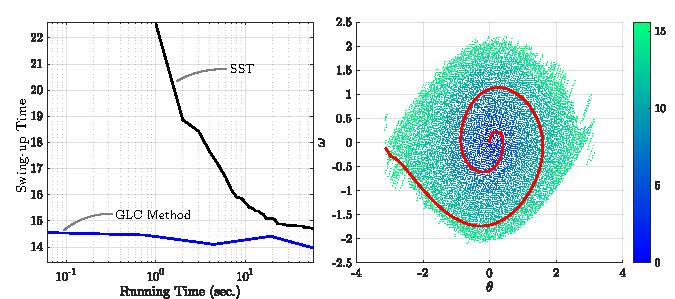
\includegraphics[width=1\textwidth]{Graphics/Pendulum_Example/pendulum}\caption{\label{fig:pendulum} (Left) Cost and running time on a logarithmic time scale of the \GLC method for resolutions $R\in\{4,5,6,7,8\}$ in blue, and the 10 trial average cost returned by SST in black. There is a notable difference in running times between the \GLC method and \SST. (Right) The colormap indicates cost and associated terminal states of signals in the set of labels $\Sigma$ at the termination of the \GLC method for $R=6$.}
\end{figure}
\end{comment}
\begin{comment}
\begin{example} (Minimum-time acrobot swing-up)
%
The acrobot is a popular system tor testing planning and control techniques.
%
It is an underactuated system with a four dimensional  state space.
%
A two-link pendulum with an actuation torque applied to the second joint emulates a gymnast swinging on a bar. 
%
The details of the dynamics can be found in~\cite{spong1995swing}. 
%

%
The model parameters are identical to those in the SST library~\cite{BBekris2015}. 
%
The goal region is the ball of radius 0.5 centered at the inverted position.
% 

%
\GLC parameters for this problem were $c=6$, $\eta(R)=16.0R^{2}$, and $h(R)=100R\log(R)$. \SST parameters are the default values in \cite{BBekris2015}. 
%
Numerical results are summarized in Figure \ref{fig:acro}.
% 
\end{example}
\end{comment}
\begin{figure}
	\centering{}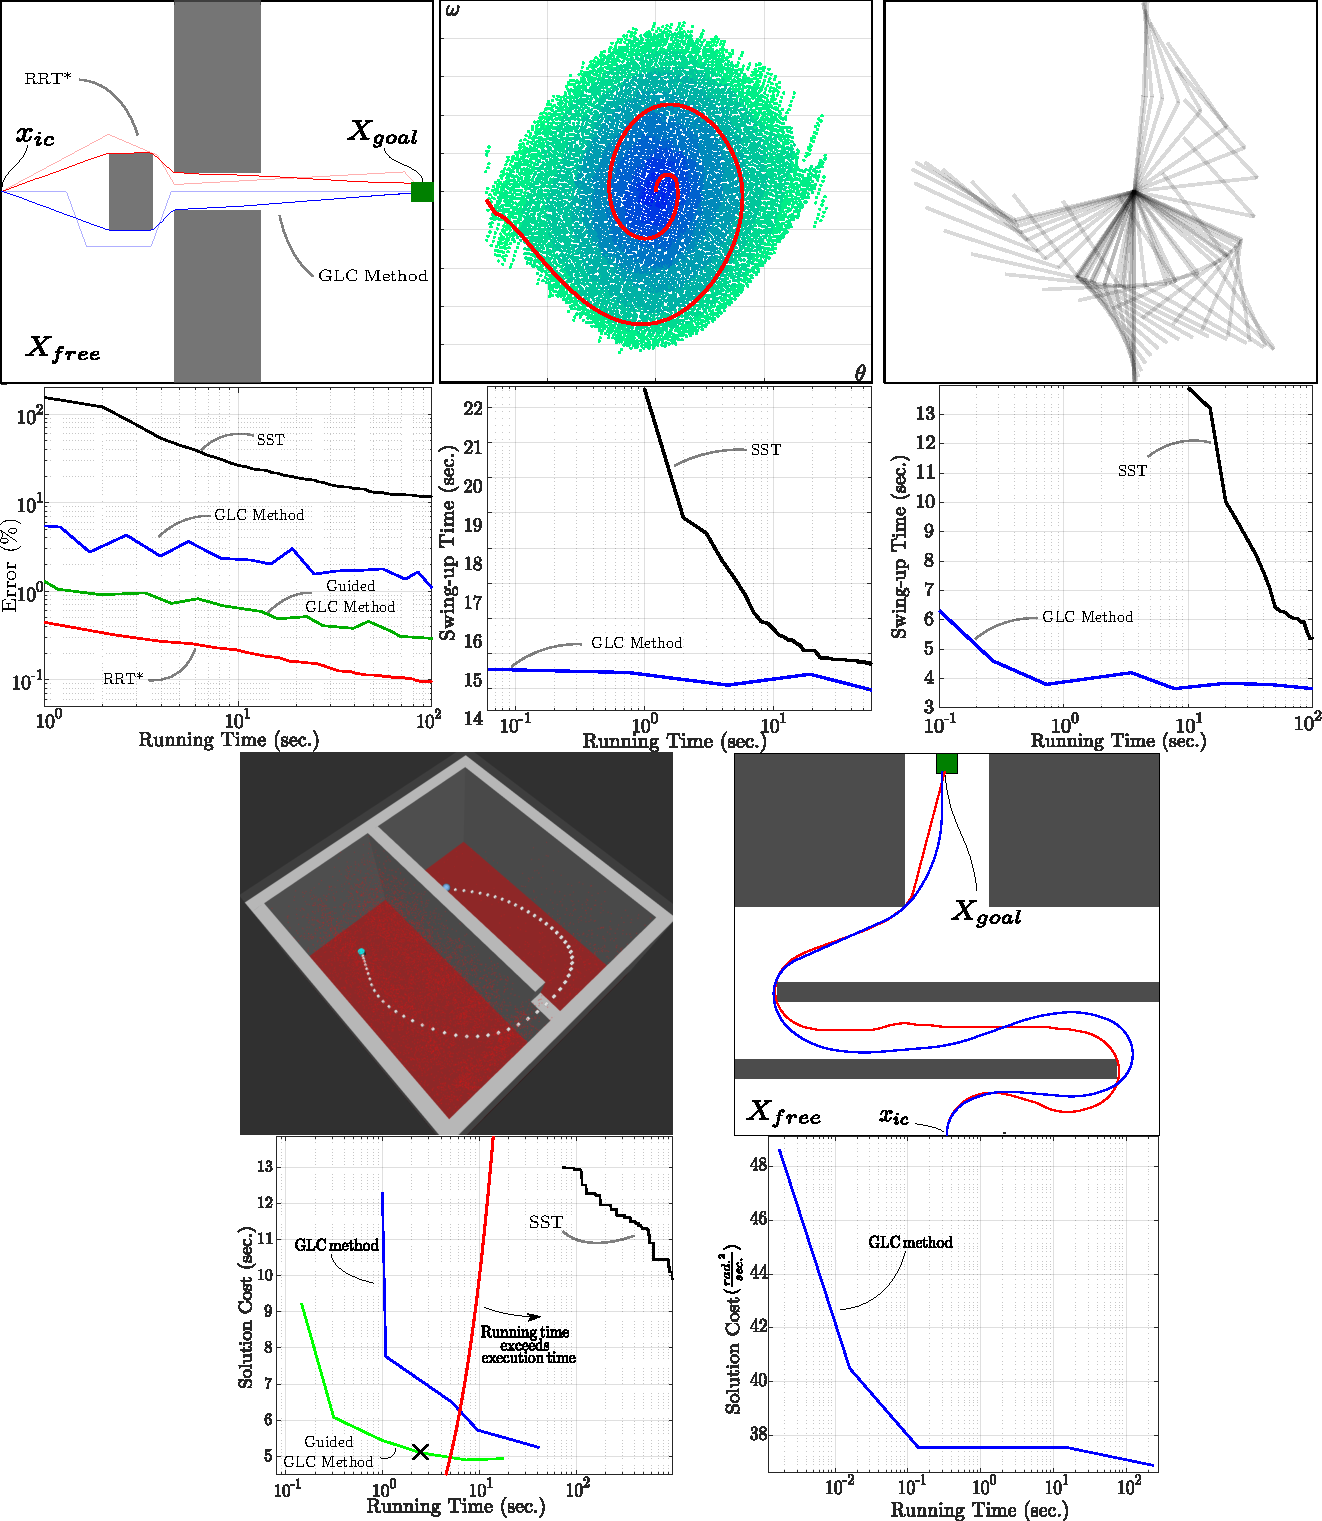
\includegraphics[width=1\textwidth]{Graphics/demos}\caption{\label{fig:bench} Running times are based on 10 trial average for randomized planners and only reported if a solution was found at a particular time in all 10 trials. {\bf Shortest path example (top-left)}; the opaque and solid paths illustrate first and last solutions obtained respectively. {\bf Pendulum example (top-middle)}; the graphic illustrates the \GLC solution for $R=7$ with the colored markers indicating the cost of grid labels. {\bf Acrobot example (top-right)}; The state space has four dimensions. Only the configuration is illustrated. {\bf Acceleration limited point robot (bottom-left)}; The graphic shows the best \GLC solution with a running time less than the execution time. The $\times$ indicates the running time of the solution in the graphic. The state space has six dimensions. Only the configuration is illustrated. {\bf Wheeled robot (bottom-right)}; The blue path indicates a \GLC solution with a quadratic angular rate penalty while the red path is a \GLC solution with a shortest path objective.}
\end{figure}
\begin{comment}
\begin{figure}
\centering{}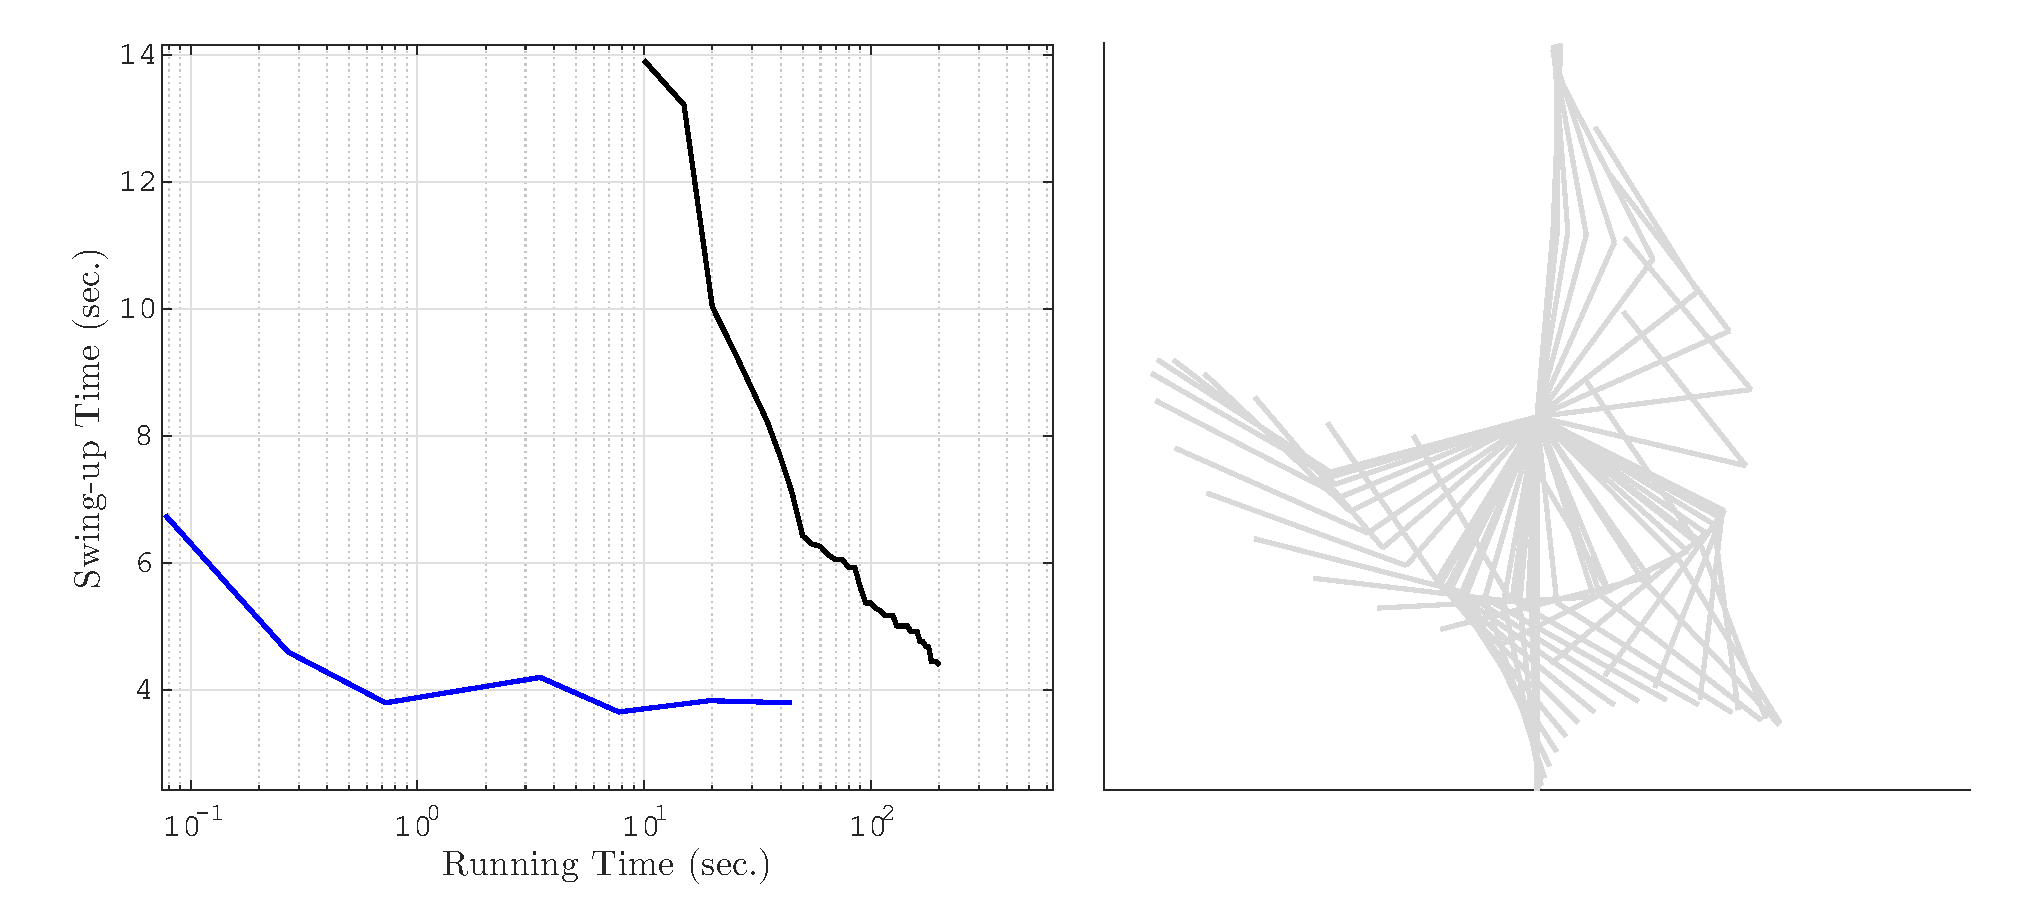
\includegraphics[width=1\textwidth]{Graphics/Acrobot_Example/acro}\caption{\label{fig:acro}(Left) Cost and running time on a logarithmic time scale of the \GLC method for resolutions $R\in\{4,...,10\}$ in blue, and the 10 trial average cost returned by SST in black. Again, there is a notable difference in running time. (Right) Snapshots of the swing-up motion
returned by the \GLC method for $R=10$.}
\end{figure}
\end{comment}
\begin{comment}
\begin{example} (Kinematic path planning)
To make a comparison with \RRTs a shortest path problem is considered.
%
The optimal local planning subroutine for \RRTs is simply the line connecting two points making \RRTs very well suited for this problem. 
%
%In other instances this may not be the case (e.g. local planning requires solving a nonlinear program). 
%

This example also investigates the guided version of the \GLC method using the \RRTs local planner's solution cost to the goal as an admissible heuristic.  

%
To fit this problem into our framework we use the model $\dot{x}=u$, with $\Omega=\{u\in\mathbb{R}^{2}:\,\Vert u\Vert_{2}=1\}$.
%
The minimum-time stage cost $g(x,u)=1$ is equivalent to a shortest path objective. 
% 

%
The parameters used for the \GLC method are $c=10$, $\eta(R)=300R^{2}$, and $h(R)=100R\log(R)$. Parameters for \SST and \RRTs are the default values for the library.
%
Numerical results are illustrated in Figure \ref{fig:kine_example}.
\begin{figure}
\centering{}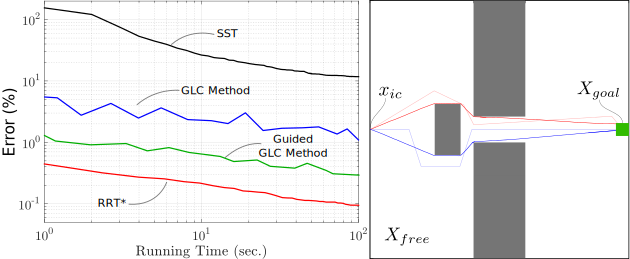
\includegraphics[width=1\textwidth]{Graphics/Kinematic_Example/kine_bench_graphic}\caption{\label{fig:kine_example} (Left) Logarithmic vertical and horizontal axis showing running time and percent error from known optimal cost. Average
running time (10 trials) for the \SST and \RRTs methods are
shown in black and red respectively. Running time of the \GLC method is shown in blue for resolutions $R\in\{20,25,...,200\}$. The guided version of the \GLC method  is shown in green. (Right) Illustration of the environment. First and last solutions returned by \RRTs are shown red while the first and last solution returned by the \GLC method are shown in blue.}
\end{figure}
\end{example}

\begin{figure}
	\centering{}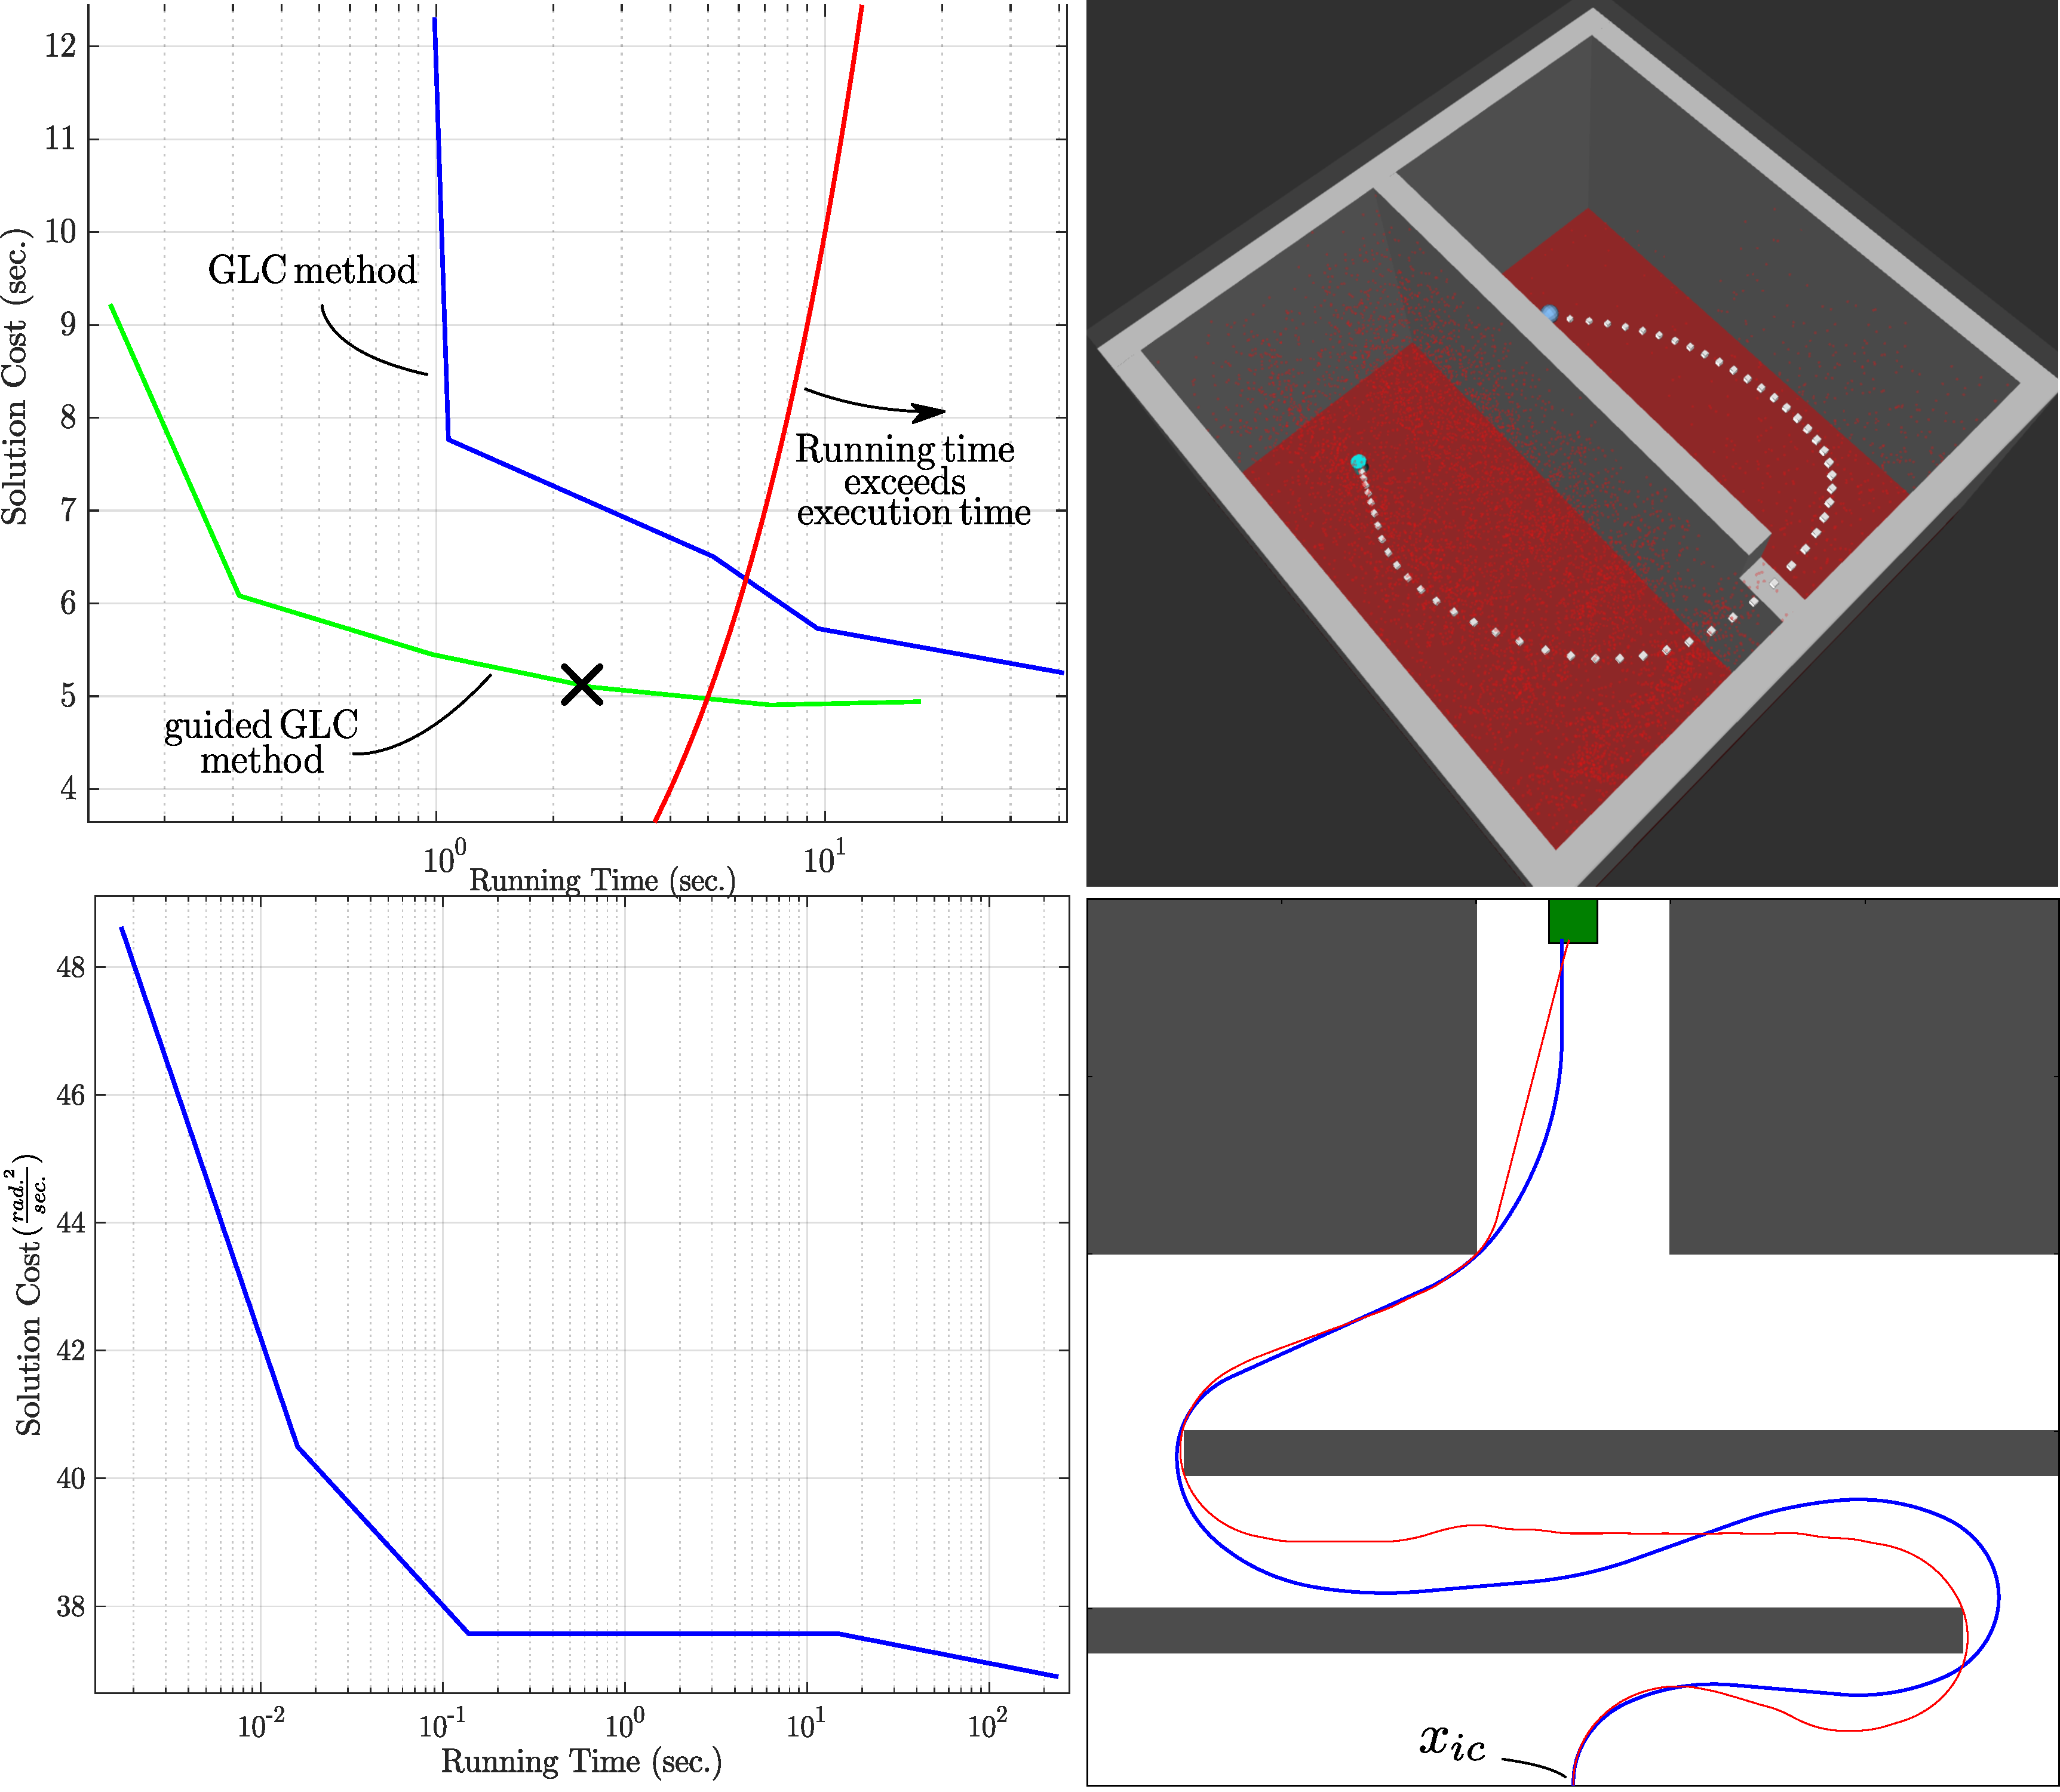
\includegraphics[width=1\textwidth]{Graphics/demos2}\caption{\label{fig:demos2} (top) Results for the acceleration limited point robot with 6 states. The red line indicates where the running time of the algorithm exceeds the execution time of the trajectory. The ${\times}$ indicates the running and execution time of the trajectory visualized on the right. (bottom) Results for the nonholonomic ground robot penalizing angular rate to reflect a rider comfort criteria. The resulting path has less abrupt cornering maneuvers.}
\end{figure}
\end{comment}


\subsection{Observations and Discussion}
%Discuss benchmarks
The \RRTs algorithm was only tested on the first example since a steering function is unavailable for the remaining four.
%
The \SST algorithm was tested in all examples but the last since neither the analysis in \cite{Li2016Asymptotically-} nor the implementation in \cite{BBekris2015} supports objectives other than minimum-time.
%

%
We observe the run-time vs. objective-cost curves for the \GLC method is several orders of magnitude faster than the \SST algorithm. 
%
In the shortest path problem, the steering function for \RRTs is a line segment between two points.
%
In this case \RRTs outperforms both the \GLC and \SST methods and is the more appropriate algorithm.  
%
A more complex steering function can increase the running time of \RRTs by a considerable constant factor making it a less competitive option. 

%Discuss realtime applications
%
In the 3D point robot example, we see the running time for the \GLC method to produce a (visually) good quality trajectory is roughly equal to the execution time.
%
This suggests six states is roughly the limit for real-time application without better heuristics. 
%

%
In the wheeled robot example a minimum time cost function was compared to a cost function which also penalized lateral acceleration.
%
The minimum time solution results in a path with abrupt changes in angular rate making it unsuitable for autonomous driving applications where passenger comfort is a consideration. 
%
Penalizing angular velocity resulted in a solution with more gradual changes in angular velocity.

Each data point in Figure \ref{fig:bench} represents the running time and solution cost of a complete evaluation of the \GLC method while \RRTs and \SST are incremental methods running until  interrupted. 
%	
Each run of Algorithm \ref{Alg} operates on $\mathcal{U}_R$ for a fixed $R$. Since $\mathcal{U}_{R}\not\subset\mathcal{U}_{R+1}$ it is possible that an optimal signal in $\mathcal{U}_R$ may be better than any signal in $\mathcal{U}_{R+1}$ for some $R$ which explains the non-monotonic convergence observed.
%
\section{\label{sec:Justification}Analysis of the GLC Condition}


%The focus of the remaining discussion is to provide intermediate results to prove that the \GLC method described by Algorithm \ref{Alg} is resolution complete.
We begin in Section \ref{sec:topology} by equipping $\mathcal{U}$ and $\mathcal{X}_{x_0}$ with metrics in order to discuss continuity of $\varphi_{x_0}$ and $J_{x_0}$. 
%
Using these metrics we can also discuss in what sense $\mathcal{U}_R$ approximates $\mathcal{U}$ in Section \ref{sec:discretization}. 
%
Finally, in Lemma \ref{lem:pruning} and Theorem \ref{thm:main}, we derive a bound on the gap between the cost of the solution output by Algorithm \ref{Alg} and the optimal cost for the problem and show that the gap converges to zero as the resolution is increased.


\subsection{Metrics on $\mathcal{X}$ and $\mathcal{U}$, and Continuity of Relevant
Maps \label{sec:topology}}

The metrics introduced by Yershov and Lavalle~\cite{yershov2011sufficient} will be used.  
%
Recall, the signal space $\mathcal{U}$ was defined in (\ref{eq:signal_space}).
A metric on this space is given by 
\begin{equation}
d_{\mathcal{U}}(u_{1},u_{2})\coloneqq\int_{[0,\min(\tau(u_{1}),\tau(u_{2})]}\Vert u_{1}(t)-u_{2}(t)\Vert_{2} \, d\mu(t)+u_{max}|\tau(u_{1})-\tau(u_{2})|.\label{eq:du}
\end{equation}
The family of trajectory spaces are now more precisely defined as 
\begin{equation}
\mathcal{X}_{x_0} \coloneqq \bigcup_{\tau>0}\left\{ x:[0,\tau]\rightarrow \mathbb{R}^n: \: x(0)=x_{0}, \, \left\Vert \frac{x(t_{1})-x(t_{2})}{|t_{1}-t_{2}|}\right\Vert _{2}\leq M\:\, \forall t_{1,2}\in[0,\tau]\right\} ,\label{eq:traj_space}
\end{equation}
where $M$ is that of assumption A-2. This set is equipped with the metric 
\begin{equation}
d_{\mathcal{X}}(x_{1},x_{2})\equiv\max_{t\in\left[0,\min\{\tau(x_{1}),\tau(x_{2})\}\right]}\left\{ \left\Vert x_{1}(t)-x_{2}(t)\right\Vert \right\} +M|\tau(x_{1})-\tau(x_{2})|.\label{eq:traj_metric}
\end{equation}

Several known continuity properties of $\varphi_{x_0}$ are reviewed here. Recall (e.g.~\cite[pg. 95]{khalil1996nonlinear}), that the distance between solutions to (\ref{eq:dynamics}) with initial conditions $x_0$ and $z_0$ is bounded by
\begin{equation}\label{lem:cont_ic}
\left\Vert [\varphi_{x_{0}}(u)](t)-[\varphi_{z_{0}}(u)](t)\right\Vert _{2}\leq\Vert x_{0}-z_{0}\Vert_{2}e^{L_{f}t}.
\end{equation}  
%
In addition to continuous dependence on the initial condition parameter, the map $\varphi_{x_{0}}$ is also continuous from $\mathcal{U}$ into $\mathcal{X}_{x_{0}}$ (cf.~\cite[Theorem 1]{yershov2011sufficient}). It is a  useful observation then that $\mathcal{X}_\mathrm{feas}$ is open when assumption A-1 is satisfied (cf.~\cite[Theorem 2]{yershov2011sufficient}) since it follows directly from the definition of continuity that $\mathcal{U}_\mathrm{feas}$ and $\mathcal{U}_\mathrm{goal}$ are open subsets of $\mathcal{U}$; recall that they are defined as the preimage of $\mathcal{X}_\mathrm{feas}$ and $\mathcal{X}_\mathrm{goal}$ under $\varphi_{x_\mathrm{ic}}$.

Similar observations for the cost functional are developed below.

\begin{lemma} \label{lem:cost_cont}
%
$J_{x_0}:\mathcal{U}\rightarrow\mathbb{R}$ is continuous for any $x_0\in \mathbb{R}^n$.
%
\end{lemma}
%
\begin{proof}
Let $u_{1},u_{2}\in\mbox{\ensuremath{\mathcal{U}}}$ and without
loss of generality, assume $\tau(u_{1})\leq\tau(u_{2})$. Denote
trajectories $\varphi_{x_{0}}(u_{1})$ and $\varphi_{x_{0}}(u_{2})$ by
$x_{1}$ and $x_{2}$ respectively. The associated difference in cost is 
\begin{equation}
\begin{array}{rl}
\left|J_{x_0}(u_{1})-J_{x_0}(u_{2})\right|= & \left|\int_{\left[0,\tau(u_{1})\right]}g\left(x_{1}(t),u_{1}(t)\right)\right.-g\left(x_{2}(t),u_{2}(t)\right)\, d\mu(t)\\
 & +\left.\int_{\left[\tau(u_{1}),\tau(u_{2})\right]}g\left(x_{2}(t),u_{2}(t)\right)\, d\mu(t)\right|.
\end{array}
\end{equation}
Using the Lipschitz constant of $g$ (cf. A-3), the definition of $d_{\mathcal{U} }$ in (\ref{eq:du}), and the definition of $d_{\mathcal{X} }$ in (\ref{eq:traj_metric}) the difference is bounded as follows: 
\begin{equation}
\begin{array}{rcl}
\left|J_{x_0}(u_{1})-J_{x_0}(u_{2})\right| & \leq & \left|\int_{\left[0,\tau(u_{1})\right]} L_{g}\left\Vert x_{1}(t)-x_{2}(t)\right\Vert _{2}\right.+L_{g}\left\Vert u_{1}(t)-u_{2}(t)\right\Vert _{2}\, d\mu(t) \\
 &  & +\left.\int_{\left[\tau(u_{1}),\tau(u_{2})\right]}g\left(x_{2}(t),u_{2}(t)\right)\, d\mu(t)\right|\\
 & \leq & L_{g}\tau(u_{1})\left\Vert x_{1}-x_{2}\right\Vert _{L_{\infty}\left[0,\tau(u_{1})\right]}+L_{g}\left\Vert u_{1}-u_{2}\right\Vert _{L_{1}\left[0,\tau(u_{1})\right]}\\
 &  & +\int_{\left[\tau(u_{1}),\tau(u_{2})\right]}\left|g\left(x_{2}(t),u_{2}(t)\right)\right|\, d\mu(t)\\
 & \leq & L_{g}\tau(u_{1}) d_{\mathcal{X}}(x_1,x_2)+ L_{g}d_{\mathcal{U}}(u_1,u_2)\\ 
& &  +\int_{\left[\tau(u_{1}),\tau(u_{2})\right]}\left|g\left(x_{2}(t),u_{2}(t)\right)\right|\, d\mu(t). 
\end{array}\label{eq:cost_diff}
\end{equation}
Since $x_2$ is continuous, $u_2$ is bounded, and $g$ is continuous, there exists a bound $G$ on $g(x_2(t),u_2(t))$ for $t\in [\tau(u_1),\tau(u_2)]$. Thus, the difference in cost is further bounded by  

\begin{equation}
\begin{array}{rcl}
\left|J_{x_0}(u_{1})-J_{x_0}(u_{2})\right| & \leq & L_{g}\tau(u_{1}) d_{\mathcal{X}}(x_1,x_2) + L_{g}d_{\mathcal{U}}(u_1,u_2) +G(\tau(u_2)-\tau(u_1)). 
\end{array}
\label{eq:cost_diff2}
\end{equation}
From the continuity of $\varphi_{x_0}$, for $d_{\mathcal{U}}(u_1,u_2)$ sufficiently small the resulting trajectories will satisfy $L_{g}\tau(u_{1}) d_{\mathcal{X}}(x_1,x_2)<\varepsilon/3$. For $u_1,u_2$ additionally satisfying $d_{\mathcal{U}}(u_1,u_2)<\frac{\varepsilon u_{max}}{3G}$ and $d_{\mathcal{U}}(u_1,u_2)<\frac{\varepsilon}{3L_g}$ we have $G(\tau(u_2)-\tau(u_1))<\varepsilon/3$  and $L_{g}d_{\mathcal{U}}(u_1,u_2)<\varepsilon/3$. For such a selection of $u_1,u_2$, we have $|J_{x_0}(u_1)-J_{x_0}(u_2)|<\varepsilon$. Thus, $J_{x_0}$ is continuous.
\qed
\end{proof} 
\begin{lemma}
\label{lem:cost_sensitivity}For any $u\in\mathcal{U}_\mathrm{feas}$ and
$x_{0},z_{0}\in\mathbb{R}^{n}$, 
\begin{equation}
|J_{x_{0}}(u)-J_{z_{0}}(u)|\leq\Vert x_{0}-z_{0}\Vert_{2}\cdot\frac{L_{g}}{L_{f}}\left(e^{L_{f}\tau(u)}-1\right)\label{eq:cost_sensitivity}
\end{equation}
\end{lemma}
\begin{proof}
The difference is bounded using the Lipschitz continuity of $g$. This is further bounded using (\ref{lem:cont_ic}). Denoting $x(t)=\varphi_{x_{0}}(u)$ and $z(t)=\varphi_{z_{0}}(u)$,
\begin{equation}
\begin{array}{rcl}
|J_{x_{0}}(u)-J_{z_{0}}(u)| & = & \left|\int_{[0,\tau(u)]}g(x(t),u(t))\right. \left.-g(z(t),u(t))\, d\mu(t) \right|\\
 & \leq & \int_{[0,\tau(u)]}\left|g(x(t),u(t))\right. \left.-g(z(t),u(t))\right|\, d\mu(t)\\
 & \leq & \int_{[0,\tau(u)]}L_{g}\left\Vert x(t)-z(t)\right\Vert _{2}\, d\mu(t)\\
 & \leq & \int_{[0,\tau(u)]}\Vert x_{0}-z_{0}\Vert_{2} L_{g}e^{L_{f}t}\, d\mu(t)\\
 & = & \Vert x_{0}-z_{0}\Vert_{2}\frac{L_{g}}{Lf}\left(e^{L_{f}\tau(u)}-1\right).
\end{array}
\end{equation}
 \qed
\end{proof}

\subsection{Properties of the Approximation of $\mathcal{U}$ by $\mathcal{U}_{R}$ \label{sec:discretization}}

%The next two results examine in what sense elements of %$\mathcal{U}$ are approximated by elements of %$\mathcal{U}_R$, and together with the continuity of the cost function, how these signals can approximate the optimal cost. 

Note that Lemma \ref{lem:density} is not a statement about the dispersion of $\mathcal{U}_R$ in $\mathcal{U}$ which does not actually converge. For numerical approximations of function spaces the weaker statement that $\limsup_{R\rightarrow \infty}\mathcal{U}_R$ is dense in $\mathcal{U}$ will be sufficient. Equivalently,
%
\begin{lemma}
\label{lem:density}For each $u\in\mathcal{U}$ and $\varepsilon>0$,
there exists $R^{*}>0$ such that for any $R>R^{*}$ there exists
$w\in\mathcal{U}_{R}$ such that $d_{\mathcal{U}}(u,w)<\varepsilon$.\end{lemma}
\begin{proof}
%The signal $u$ will first be approximated by a uniformly continuous
%function $\omega$, and then $w\in\mathcal{U}_{R}$ will be constructed
%to approximate $\omega.$ 

By Lusin's Theorem~\cite[pg. 41]{kolmogorov1961elements}, there exists
a continuous $\upsilon:[0,\tau(u)]\rightarrow\Omega$ such that 
\begin{equation}
\mu(\{t\in[0,\tau(u)]:\:\upsilon(t)\neq u(t)\})<\frac{\varepsilon}{3u_{max}}.
\end{equation}
The domain of $\upsilon$ is compact so $\upsilon$ is also uniformly continuous. Denote its modulus of continuity by $\delta(\epsilon)$,
\begin{equation}
|\sigma-\gamma|<\delta(\epsilon)\Rightarrow\Vert\upsilon(\sigma)-\upsilon(\gamma)\Vert_{2}<\epsilon.
\end{equation}


To construct an approximation of $\upsilon$ by $w\in\mathcal{U}_{R}$
choose $R$ sufficiently large so that (i) $h(R)/R>\tau(u)$,
(ii) there exists an integer $r$ such that $0<\tau(u)-r/R<1/R<\delta\left(\frac{\varepsilon}{6\tau(u)}\right)$,
and (iii) the dispersion of $\Omega_{R}$ in $\Omega$ is less than $\frac{\varepsilon}{6\tau(u)}$. 

Then for $t\in[(i-1)/R,i/R)$ $i=1,...,r$ there exists ${\rm v}_{i}\in\Omega_{R}$
such that $\Vert {\rm v}_{i}-\upsilon(t)\Vert_{2}<\frac{\varepsilon}{3\tau(u)}.$
Select $w\in\mathcal{U}_{R}$ which is equal to ${\rm v}_{i}$ on
each interval. Combining (i)-(iii), 
\begin{equation}
\begin{array}{rcl}
d_{\mathcal{U}}(\upsilon,w) & = & \int_{[0,r/R]}\Vert w(t)-\omega(t)\Vert_{2},\, d\mu(t)+u_{max}|r/R-\tau(\omega)|\\
 & < & \int_{[0,r/R]}\Vert w(t)-\omega(t)\Vert_{2},\, d\mu(t)+\frac{\varepsilon}{6}\\
 & < & \int_{[0,r/R]}\frac{\varepsilon}{3\tau(u)},\, d\mu(t)+\frac{\varepsilon}{6}\\
 & < & \frac{\varepsilon}{2}.
\end{array}
\end{equation}
Thus, by the triangle inequality
\begin{equation}
d_{\mathcal{U}}(u,w)\leq d_{\mathcal{U}}(u,\upsilon)+d(\upsilon,w)<\varepsilon.
\end{equation}
\qed
\end{proof}

We use $cl(\cdot)$ and $int(\cdot)$ to denote the closure and interior of subsets of $\mathcal{U}$.
\begin{lemma}
\label{lem:no_limit_points}For any $w\in cl\left(int\left(\mathcal{U}_\mathrm{goal}\right)\right)$
and $\varepsilon>0$ there exists $R^{*}>0$ such that for any $R>R^{*}$
\begin{equation}
\min_{u\in\mathcal{U}_{R}\cap\mathcal{U}_\mathrm{goal}}\left\{ \left|J_{x_\mathrm{ic}}(u)-J_{x_\mathrm{ic}}(w)\right|\right\} <\varepsilon.
\end{equation}
\end{lemma}
\begin{proof}
$\omega\in cl\left(int\left(\mathcal{U}_\mathrm{goal}\right)\right)$ implies
that for all $\delta>0$, $B_{\delta/2}(\omega)\cap int(\mathcal{U}_\mathrm{goal})\neq\emptyset$.
Then each $\upsilon\in int(\mathcal{U}_\mathrm{goal})$ has a neighbourhood
$B_{\rho}(\upsilon)\subset int(\mathcal{U}_\mathrm{goal})$ with $\rho<\frac{\delta}{2}$.
Take $\upsilon\in B_{\delta/2}(\omega)\cap int(\mathcal{U}_{goal.})$.
By Lemma \ref{lem:density}, for sufficiently large $R$, there exists $u\in\mathcal{U}_{R}$ such
that $d_{\mathcal{U}}(\upsilon,u)<\delta/2$ which implies $u\in B_{\rho}(\upsilon)\subset int(\mathcal{U}_\mathrm{goal})$.
Then $u\in\mathcal{U}_\mathrm{goal}$ and $d_{\mathcal{U}}(\omega,u)<d_{\mathcal{U}}(\omega,\upsilon)+d_{\mathcal{U}}(\upsilon,u)<\delta$. Now by the continuity of $J_{x_\mathrm{ic}}$ for $\delta$ sufficiently small, $d_{\mathcal{U}}(\omega,\upsilon)<\delta$ implies $|J_{x_\mathrm{ic}}(u)-J_{x_\mathrm{ic}}(w)| <\varepsilon$ from which the result follows.
\qed
\end{proof}
A sufficient condition for every $\omega\in\mathcal{U}_\mathrm{goal}$ to
be contained in the closure of the interior of $\mathcal{U}_\mathrm{goal}$ is that $\mathcal{U}_\mathrm{goal}$ be open which is the case when Assumption A-1 is satisfied. 
%
%In connection to the framework of %~\cite{karaman2011sampling,Li2016Asymptotically-}, a problem is %$\delta$-robustly feasible iff $cl(int(\mathcal{U}_\mathrm{goal}))\neq %emptyset$.    


\subsection{Pruning $\mathcal{U}_{R}$ with the GLC Condition \label{sec:pruning}}

To describe trajectories remaining on the $\varepsilon$-interior of $X_\mathrm{free}$ at each instant and which terminate on the $\varepsilon$-interior of $X_\mathrm{goal}$ the following sets are defined,
\begin{equation}
\begin{array}{l}
\mathcal{X}_\mathrm{goal}^{\varepsilon}\coloneqq\left\{ x\in\mathcal{X}_\mathrm{goal}:\,\; B_{\varepsilon}(x(t))\subset X_\mathrm{free}\, \forall t\in[0,\tau(x)], \, B_{\varepsilon}(x(\tau(x))\subset X_\mathrm{goal}\right\} ,\\
\mathcal{U}_\mathrm{goal}^{\varepsilon}\coloneqq\left\{ u\in\mathcal{U}_\mathrm{goal}:\,\varphi_{x_\mathrm{ic}}(u)\in\mathcal{X}_\mathrm{goal}^{\varepsilon}\right\} ,
\end{array}\label{eq:interiors}
\end{equation}
and similarly for $c_{R}$,
\begin{equation}
c_{R}^{\varepsilon}\coloneqq\min_{u\in\mathcal{U}_{R}\cap\mathcal{U}_\mathrm{goal}^{\varepsilon}}\left\{ J_{x_\mathrm{ic}}(u)\right\} .\label{eq:cr_ep}
\end{equation}
 Since $\ensuremath{\mathcal{U}_\mathrm{goal}^{\varepsilon}\subset\mathcal{U}_\mathrm{goal}}$
we have that $0\leq c_{R}\leq c_{R}^{\varepsilon}$. 
\begin{lemma}
\label{lem:approx_equal_optimal}If $\lim_{R\rightarrow\infty}\epsilon(R)=0$
then $\lim_{R\rightarrow\infty}c_{R}^{\epsilon(R)}=c^{*}$.\end{lemma}
\begin{proof}
By the definition of $c^{*}$ in (\ref{eq:meaningful_problem}), for any
$\varepsilon>0$ there exists $\omega\in\mathcal{U}_\mathrm{goal}$ such
that $J_{x_\mathrm{ic}}(\omega)-\varepsilon/2<c^{*}$. Since
$\mathcal{U}_\mathrm{goal}$ is open and $\varphi_{x_\mathrm{ic}}$ is continuous there exists $\tilde{r}>0$ and $\rho>0$
such that $B_{\tilde{r}}(\omega)\subset\mathcal{U}_\mathrm{goal}$ and $\varphi_{x_\mathrm{ic}}(B_{\tilde{r}}(\omega))\subset B_{\rho}(\varphi_{x_\mathrm{ic}}(\omega))$.
Thus, $\omega\in\mathcal{U}_\mathrm{goal}^{\tilde{r}}$. Similarly, there exists a positive $r<\tilde{r}$ such that $\varphi_{x_\mathrm{ic}}(B_{r}(\omega))\subset B_{\rho/2}(\varphi_{x_\mathrm{ic}}(\omega))$
and $B_{r}(\omega)\subset\mathcal{U}_\mathrm{goal}^{\rho/2}$. From the continuity
of $J$ in Lemma \ref{lem:cost_cont} there also exists a positive
$\delta<r$ such that for any signal $\upsilon$ with $d_{\mathcal{U}}(\upsilon,\omega)<\delta$
we have $|J_{x_\mathrm{ic}}(\omega)-J_{x_\mathrm{ic}}(\upsilon)|<\varepsilon/2$.

Next, choose $R^{*}$ to be sufficiently large such that $R>R^*$ implies $\mbox{\ensuremath{\epsilon}}(R)<\rho/2$
and $B_{\delta}(\omega)\cap\mathcal{U}_{R}\neq\emptyset$. Such a resolution $R^{*}$ exists by
Lemma \ref{lem:no_limit_points} and the assumption $\lim_{R\rightarrow\infty}\epsilon(R)=0$.
Now choose $u\in B_{\delta}(\omega)\cap\mathcal{U}_{R}$.
Then $|J_{x_\mathrm{ic}}(u)-J_{x_\mathrm{ic}}(\omega)|<\varepsilon/2$ and $u\in\mathcal{U}_\mathrm{goal}^{\rho/2}\subset\mathcal{U}_\mathrm{goal}^{\epsilon(R)}$.
Then by definition of $c_{R}^{\epsilon(R)}$, $u\in\mathcal{U}_\mathrm{goal}^{\epsilon(R)}$
implies $c_{R}^{\epsilon(R)}\leq J_{x_\mathrm{ic}}(u)$. Finally, by triangle
inequality, 
\begin{equation}
|J_{x_\mathrm{ic}}(u)-c^{*}|<|J_{x_\mathrm{ic}}(u)-J_{x_\mathrm{ic}}(\omega)|+|J_{x_\mathrm{ic}}(\omega)-c^{*}|<\varepsilon.
\end{equation}
Rearranging the expression yields $J_{x_\mathrm{ic}}(u)<c^{*}+\varepsilon$
and thus, $c_{R}^{\epsilon(R)}<c^{*}+\varepsilon$. The result follows
since the choice of $\varepsilon$ is arbitrary.
\qed
\end{proof}

To simplify the notation in what follows, a concatenation operation on elements of $\mathcal{U}$ is defined.
For $u_{1},u_{2}\in\mathcal{U}$, their concatenation $u_{1}u_{2}$
is defined by 
\begin{equation}
[u_{1}u_{2}](t)\coloneqq\left\{ \begin{array}{c}
u_{1}(t),\, t\in[0,\tau(u_{1}))\\
u_{2}(t-\tau(u_{1})),\, t\in[\tau(u_{1}),\tau(u_{1})+\tau(u_{2})]
\end{array}\right..\label{eq:concatenation}
\end{equation}
%
The concatenation operation will be useful together
with the following equalities which are readily verified, 
\begin{equation}\label{eq:cost_homo}
J_{x_{0}}(u_{1}u_{2})=J_{x_{0}}(u_{1})+J_{[\varphi_{x_0}(u_1)](\tau(u_1))}(u_{2})
\end{equation}
\begin{equation}
\ensuremath{\varphi_{x_{0}}(u_{1}u_{2})=\varphi_{x_{0}}(u_{1})\varphi_{[\varphi_{x_{0}}(u_1)](\tau(u))}(u_{2})}.\label{eq:x_concat}
\end{equation}
The concatenation operation on $\mathcal{X}_{x_{0}}$ in (\ref{eq:x_concat})
is defined in the same way as in (\ref{eq:concatenation}). 
%

%
\begin{lemma}
\label{lem:pruning}Let $\delta_0=\frac{\sqrt{n}}{\eta(R)}e^{\frac{L_{f}h(R)}{R}}$.
For $\varepsilon\geq \delta_0$ and $u_{i},u_{j}\in\mathcal{U}_{R}\cap\mathcal{U}_\mathrm{feas}$, if
$u_{i}\prec_{R}u_{j}$, then for each descendant of $u_{j}$ in $\mathcal{U}_\mathrm{goal}^{\varepsilon-\delta_0}$
with cost $c_{j}$, there exists a descendant of $u_{i}$ in $\mathcal{U}_\mathrm{goal}$
with cost $c_{i}\leq c_{j}$.\end{lemma}
\begin{proof}
Suppose there is a $w\in\mathcal{U}_{R}$ such that $u_{j}w\in\mathcal{U}_{R}$
is a descendant of $u_{j}$ and $u_{j}w\in\mathcal{U}_\mathrm{goal}^{\varepsilon}.$
 Since $u_{i}\overset{R}{\sim}u_{j}$,
\begin{equation}
\left\Vert[\varphi_{x_\mathrm{ic}}(u_{i}w)](\tau(u_{i}))-[\varphi_{x_\mathrm{ic}}(u_{j}w)](\tau(u_{j}))\right\Vert_2\leq \frac{\sqrt{n}}{\eta(R)}.
\end{equation}
Then, by equation (\ref{lem:cont_ic}), for all $t\in[0,\tau(w)]\subset[0,h(R)/R]$, 
\begin{equation}
\Vert[\varphi_{x_\mathrm{ic}}(u_{i}w)](t+\tau(u_{i}))-[\varphi_{x_\mathrm{ic}}(u_{j}w)](t+\tau(u_{j}))\Vert\leq\frac{\sqrt{n}}{\eta(R)}e^{\frac{L_{f}h(R)}{R}}.\label{eq:-8}
\end{equation}
Then for $\delta_0=\frac{\sqrt{n}}{\eta(R)}e^{\frac{L_{f}h(R)}{R}}$
we have $u_{i} w \in \mathcal{U}_\mathrm{goal}^{\varepsilon-\delta_0}.$ 
As for the cost, from equation (\ref{eq:cost_homo}) 
\begin{equation}
\begin{array}{rcl}
J_{x_\mathrm{ic}}(u_{i} w) & = & J_{x_\mathrm{ic}}(u_{i})+J_{[\varphi_{x_\mathrm{ic}}(u_{i})](\tau(u_{i}))}(w)\\
 & \leq & J_{x_\mathrm{ic}}(u_{j})+\frac{\sqrt{n}}{\eta(R)}\frac{L_{g}}{L_{f}}\left(e^{\frac{L_{f}h(R)}{R}}-1\right) +J_{[\varphi_{x_\mathrm{ic}}(u_{j})](\tau(u_{j}))}(w)\\
 & \leq & J_{x_\mathrm{ic}}(u_{j})+J_{[\varphi_{x_\mathrm{ic}}(u_{j})](\tau(u_{j}))}(w)\\
 & \leq  & J_{x_\mathrm{ic}}(u_{j}w)\\
\end{array}
\end{equation}
 The first step applies the conditions for $u_{i}\prec_{R}u_{j}$.
The second step combines Lemma \ref{lem:cost_sensitivity} and $u_{i}\overset{N}{\sim}u_{j}$. 
\qed
\end{proof}
In the above Lemma, the quantity $\delta_0$ was constructed based on the radius of the partition of $X_\mathrm{free}$ and the sensitivity of solutions to initial conditions. 
%
%
Let $\delta_k$ be defined as a finite sum of related quantities, $\delta_k\coloneqq\sum_{i=1}^{k}\frac{\sqrt{n}}{\eta(R)}e^{\frac{L_{f}(h(R)-i)}{R}}$. The following bound will be useful to state our main result in the next Theorem,
\begin{equation}
\delta_{h(R)}=\sum_{i=1}^{h(R)}\frac{\sqrt{n}}{\eta(R)}e^{\frac{L_{f}(h(R)-i)}{R}} \leq\frac{R\sqrt{n}}{L_{f}\eta(R)}\left(e^{L_{f}h(R)/R}-1\right).\label{eq:inequality}
\end{equation}
This is derived as follows 
\begin{equation}
\begin{array}{rcl}
\sum_{i=1}^{h(R)}\frac{\sqrt{n}}{\eta(R)}e^{\frac{L_{f}(h(R)-i)}{R}} & = & \frac{\sqrt{n}}{\eta(R)}\sum_{i=0}^{h(R)-1}e^{\frac{L_{f}i}{R}}\\
 & \leq & \frac{\sqrt{n}}{\eta(R)}\int_{0}^{h(R)}e^{\frac{L_{f}}{R}\rho}d\rho\\
 & = & \frac{R\sqrt{n}}{L_{f}\eta(R)}\left(e^{\frac{L_{f}h(R)}{R}}-1\right).
\end{array}
\end{equation}
\begin{theorem}\label{thm:main}
Let $\epsilon(R)=\frac{R\sqrt{n}}{L_{f}\eta(R)}\left(e^{\frac{L_{f}h(R)}{R}}-1\right)$. Algorithm \ref{Alg} terminates in finite time and returns a solution with cost less than or equal to $c^{\epsilon(R)}_R$.
\end{theorem}
%
\begin{proof}
The queue is a subset of $\mathcal{U}_R\cup \{Id_\mathcal{U} \}$ and at line 3 in each iteration a lowest cost signal $u$ is removed from the queue. 
%
In line 13, only children of the current signal $u$ are added to the queue. Since $\mathcal{U}_R$ is organized as a tree and has no cycles, any signal $u$ will enter the queue at most once.
%Observe that any $w$ from the finite set $\mathcal{U}_R$ enters the queue at most once since $w$ is not a descendant of itself and only children of $w$ enter the queue in line 13. 
%
Therefore the queue must be empty after a finite number of iterations so the algorithm terminates.

Next, as a point of contradiction consider the hypothesis that the output has cost greater than $c_R^{\epsilon(R)}$. 
%
Then $c_R^{\epsilon(R)}<\infty$ and by the definition of  $c_R^{\epsilon(R)}$  in (\ref{eq:cr_ep}), it is necessary that $\mathcal{U}_{R}\cap \mathcal{U}_\mathrm{goal}^{\epsilon(R)}$ is non-empty. 

Signals $u_0\in \mathcal{U}_{R}\cap\mathcal{U}_\mathrm{goal}^{\epsilon(R)}$ with cost $J_{x_\mathrm{ic}}(u_0)=c_R^{\epsilon(R)}$ are descendants of $Id_\mathcal{U}$ which is initially present in the queue. 
%
The hypothesis prohibits these signals from entering the queue. Otherwise, by (\ref{eq:queue}) they would be evaluated before any signal of cost greater than $c_R^{\epsilon(R)}$.To prevent these signals from entering the queue a signal $u_1$  with $depth(u_1)\geq 1$ must at some iteration be present in $\Sigma$ with $u_1 \prec_R a_0$ for an ancestor $a_0$ of each $u_0$. 
%
By line 10, having $u_1$ present in $\Sigma$ allows signals in the sub-tree rooted at $a_0$ containing each $u_0$ to be prevented from entering the queue. 
%
From Lemma \ref{lem:pruning}, each $u_1$ has a descendant in $\mathcal{U}_R$ of the form $u_1d_1$ such that $u_1d_1\in \mathcal{U}_\mathrm{goal}^{\epsilon(R)-\delta_1}$ and $J_{x_\mathrm{ic}}(u_1d_1)\leq c_R^{\epsilon(R)-\delta_1}$. 
%
To be present in $\Sigma$, a signal $u_1$ must at some point be present in the queue as well by line 10. 
%
The hypothesis implies that $u_1d_1$ does not enter the queue which is only possible by the same mechanism as for $u_0$.
%
%The signal $u_1$ must at some point enter the queue since $u_1\in\Sigma$ (line 13). but the hypothesis implies that some ancestor $a_2$ of $u_1d_1$ with $depth(a_1)\geq 2$ must be discarded in the same way as $u_0$

%Since $u_1\in\Sigma$, it must at some point enter the queue (line 13). 
%
%With a descendant violating the hypothesis, there at some point must exist $u_2\in \Sigma $ with $depth(u_2)\geq 2$ such that $u_2\prec_R a_2$ for some ancestor $a_2$ of $u_1d_1$ so that the sub-tree rooted at $u_1d_1$ does not enter the queue. 
%
%Again by Lemma \ref{lem:pruning} each such $u_2$ has a descendant $u_2d_2\in\mathcal{U}_\mathrm{goal}^{\epsilon(R)-\delta_2}$ with $J(u_2d_2,x_\mathrm{ic})\leq c_R^{\epsilon(R)}$. 

Suppose that repeating the process $k<h(R)$ times reveals that a signal $u_k$ with $depth(u_k)\geq k$ must at some iteration be present in the queue and that there is a descendant  $u_kd_k\in\mathcal{U}_R\cap\mathcal{U}_\mathrm{goal}^{\epsilon(R)-\delta_k}$  with cost $J_{x_\mathrm{ic}}(u_kd_k)\leq c_R^{\epsilon(R)}$.
%
Note, $\delta_k \leq \epsilon(R) $ for any $k \leq h(R)$ by (\ref{eq:inequality}).
%
The hypothesis implies that an ancestor $a_{k}$ of $u_kd_k$ must be prevented from entering the queue in lines 9-10 by evaluating $u_{k+1}\prec_R a_{k}$ for some $u_{k+1}\in \Sigma$ with $depth(u_{k+1})\leq k+1$. 
%
Again, by Lemma \ref{lem:pruning}, a descendant of $u_{k+1}$ of the form $u_{k+1}d_{k+1}$ will be in $\mathcal{U}^{\epsilon(R)-\delta_{k+1}}_\mathrm{goal}$ with cost $J_{x_\mathrm{ic}}(u_{k+1}d_{k+1})\leq c_R^{\epsilon(R)-\delta_{k+1}}$ so that some anscestor of $u_{k+1}d_{k+1}$ must be prevented from entering the queue. 

By induction on $k$ we conclude that this procedure can continue up to $k=h(R)$ at which point we find it necessary that there exist signals $u_{h(R)}$ with $depth(u_{h(R)})= h(R)$ such that $u_{h(R)}\prec_R u_{h(R)-1}d_{h(R)-1}$ for the descendant of $u_{h(R)-1}$ in $\mathcal{U}^{\epsilon(R)-\delta_{h(R)-1}}_\mathrm{goal}$. By Lemma \ref{lem:pruning} $u_{h(R)}\prec_R u_{h(R)-1}d_{h(R)-1}$ implies $u_{h(R)}$ has a descendant in $\mathcal{U}_\mathrm{goal}$. However, $u_{h(R)}$ has no descendants; a contradiction.   


\qed
\end{proof}
%

The choice of $\epsilon(R)$ in Theorem \ref{thm:main} converges to zero by  (\ref{eq:partition_scaling}).
%
Then by Lemma \ref{lem:approx_equal_optimal} we have $c_{R}^{\epsilon(R)}\rightarrow c^{*}$. 
%
An immediate corollary is that the \GLC method is resolution complete which is the main contribution of this work stated in Theorem \ref{thm:informal}.

\section{Conclusion\label{sec:Conclusions}}
%
In this paper we described a simple grid-based approximation of the optimal kinodynamic motion planning problem and developed the appropriate generalization of label correcting methods to efficiently search the approximation.
%
The advantage of the \GLC method is that it does not require a point-to-point local planning subroutine. 
%
Moreover, numerical experiments demonstrate that the \GLC method is considerably faster the related \SST algorithm, and is more broadly applicable than the \RRTs algorithm. 

%Our purpose has been to develop an optimal kinodynamic motion planning algorithm that is computationally efficient, provably resolution complete, and does not require a local planning subroutine. 
%
%Inspired by the effectiveness of label correcting methods, efficiency was achieved by generalizing the labeling technique with the \GLC conditions. 

The focus of the paper, and its main contribution was the theoretical investigation showing that the cost of the feasible solutions returned by the \GLC method converge to the optimal cost for the problem.
%

%
From a practical point of view the proposed algorithm is easy to implement and may be used directly for motion planning and trajectory optimization.
%
Future investigations will include convergence rate analysis, improved partitioning schemes over the hypercube grid we presented, and the construction of admissible heuristics for kinodynamic motion planning to guide the search.
\pagebreak
\section*{Acknowledgements}
This research was funded in part by the Israeli Ministry of Defense. 
%

%
We are also grateful to our colleagues Michal \v C\'ap and Dmitry Yershov for their insightful comments. 
\bibliographystyle{splncs}
\bibliography{references}

\end{document}